\chapter{One-dimensional finite-volume methods}
\label{chp-1d-fv}

\theoremstyle{plain}
\newtheorem{lema}{Lemma}[chapter]

\theoremstyle{plain}
\newtheorem{prop}{Proposition}[chapter]

\theoremstyle{plain}
\newtheorem{thrm}{Theorem}[chapter]

\theoremstyle{plain}
\newtheorem{remark}{Remark}[chapter]

\theoremstyle{plain}
\newtheorem{corollary}{Corollary}[chapter]

\theoremstyle{plain}
\newtheorem{definition}{Definition}[chapter]

The aim of this chapter is to provide a detailed description of one-dimensional (1D)
finite-volume (FV) schemes within a Semi-Lagrangian (SL) framework, specifically applied
to the 1D advection equation with periodic boundary conditions. To introduce the FV-SL
schemes, we begin by discretizing the spatial and temporal domains into uniform grids.
Subsequently, the FV-SL schemes involve three steps.

The first step involves computing the departure points of the spatial grid edges.
The second step, known as reconstruction, utilizes the grid cell average values to
determine a piecewise function within each cell. This piecewise function approximates the
values of the advected quantity and ensures the preservation of its local mass within each grid cell.
The third step entails updating the fluxes at the grid edges by integrating the reconstruction
function over a domain that extends from the departure point of the grid edge to the grid edge itself.

The first step of FV-SL schemes can be accomplished by integrating an ordinary differential
equation backward in time.
The second step is performed using the Piecewise-Parabolic Method (PPM) proposed by \citet{colella:1984}.
As the name suggests, PPM employs piecewise-parabolic functions.
The third and final step is computed exactly, as the reconstruction functions consist of parabolas that preserve the local mass.

It is worth noting that the reconstruction function can be constructed using functions other than parabolas. In fact, the Piecewise-Parabolic Method (PPM) can be seen as an
extension of the Piecewise-Linear method proposed by \citet{vanleer:1977}, which,
in turn, was inspired by the Piecewise-Constant method introduced by \citet{godunov:1959}. 
Additionally, other schemes inspired by PPM have been proposed in the literature utilizing
higher-order polynomials, such as quartic polynomials \citep{white:2008}. For a
comprehensive review of general piecewise-polynomial reconstruction, we recommend
referring to the technical report by \citet{engwirda:2016}, \citet{lauritzen:2011}, and the
references therein.

The PPM approach has become popular in the literature for gas dynamics simulations, astrophysical 
phenomena modeling \citep{woodward:1986}, and later on atmospheric simulations \citep{carpenter:1990}. 
Indeed, PPM has been implemented in the FV3 dynamical core on its latitude-longitude grid \citep{lin:2004}
and cubed-sphere \citep{putman:2007} versions.
Although many other shapes for the basis functions and higher-order schemes are available in the literature, 
\citet{harris:2021} points out that the PPM scheme suits the needs of FV3 well. It is a flexible method that
can be modified to ensure low diffusivity or shape preservation, for example.
Additionally, a finite-volume numerical method usually requires monotonicity constraints, which, according 
to Godunov's theorem, limit the order of convergence to at most 1. 
Therefore, a higher-order scheme needs to strike a well-balanced trade-off between increasing computational 
cost and potential benefits.

This chapter starts with a basic review of one-dimensional conservation laws in
the integral form in Section \ref{chp2-sec1}, and in Section \ref{chp2-sec2} 
we set the framework of general one-dimensional finite-volumes schemes,
where we also introduce concepts such as consistency, convergence and stability.
Section \ref{chp2-sec-ppm} describes the PPM method and its convergence order analysis
of its reconstruction in given in Subsection \ref{chp2-sec-recon}.
Subsection \ref{chp2-sec-mono} is dedicated to introducing possible ways to monotonize
the parabolas.
Subsection \ref{chp2-sec-flux} is dedicated to the description and investigation of the PPM flux
computation considering the one-dimensional advection equation as the conservation law.
Section \ref{chp2-sec-numerical-exp} shows some numerical results using the PPM scheme
for the advection equation.  At last, Section \ref{chp2-sec-conclusion} presents
some conclusions.
The usage of PPM to solve two-dimensional problems
will be addressed in Chapter \ref{chp-2d-fv}.

\section{One-dimensional advection equation in integral form}
\label{chp2-sec1}
\subsection{Notation}
\label{chp2-sec-not}
Before introducing the FV-SL schemes, let us establish some notation by introducing
the concepts of a $\Delta x$-grid, a $\Delta t$-temporal grid, and the
$(\Delta x, \Delta t, \lambda)$-discretization, as well as the concept of grid function/winds.
\begin{definition}[$\Delta x$-grid]
	For a given interval $\Omega = [a,b]$ and a positive real number $\Delta x$ such that 
    $\Delta x = (b-a)/N$ for some positive integer $N$, 
	we say that $\Omega_{\Delta x}= \{X_i \}_{i=1}^{N}$ is a $\Delta x$-grid for $[a,b]$ if
	\begin{align*}
        X_i = [x_{i-\frac{1}{2}}, x_{i+\frac{1}{2}}],
	    \quad a = x_{\frac{1}{2}} < x_{\frac{3}{2}} < \cdots < x_{N-\frac{1}{2}} < x_{N+\frac{1}{2}} = b,
    \end{align*}
	and $\Delta x = x_{i+\frac{1}{2}} - x_{i-\frac{1}{2}}$. 
	Each $X_i$ is referred to as a control volume or cell, and $x_{i-\frac{1}{2}}$ and 
	$x_{i+\frac{1}{2}}$ are the edges of the control volume $X_i$.
	The cell centroid is defined by
    \begin{align*}
    x_i = \frac{1}{2}(x_{i+\frac{1}{2}} + x_{i-\frac{1}{2}}),\quad \forall i = 1, \cdots, N,
    \end{align*}
	and $\Delta x$ is the cell length.
\end{definition}
\begin{remark}
	We may extend the definition of cells $X_i$ for values of $i$ outside the range $1,\cdots,N$ as $X_i = [a+(i-1)\Delta x, a+i\Delta x]$.
	These cells are known as ghost cells.
\end{remark}
\begin{definition}[$\Delta t$-temporal grid]
	For a given interval $[0,T]$ and a positive real number $\Delta t$ such that $\Delta t = T/N_T$
    for some positive integer $N_T$, we say that  $T_{\Delta T}= \{T_n\}_{n=0}^{N_T}$ a $\Delta t$-temporal grid for $[0,T]$ if
    \begin{align*}
	T_n = [t^n, t^{n+1}], \quad t^n = n\Delta t, \quad \Delta t = \frac{T}{N_T}, \quad \forall n = 0, \cdots, N_T.
    \end{align*}
\end{definition}
\begin{definition}[$(\Delta x,\Delta t, \lambda)$-discretization]
\label{chp2-def-dxtimegrid}
	Given $\Omega \times [0,T]$, $\Omega = [a,b]$ and positive real numbers $\Delta x$ and $\Delta t$,
    we say that $(\Omega_{\Delta x}, T_{\Delta t})$ is a $(\Delta x, \Delta t, \lambda)$-discretization 
    of $\Omega \times [0,T]$ if $\Omega_{\Delta x}$ is a $\Delta x$-grid for $\Omega$, 
    ${T}_{\Delta t}$ is a $\Delta t$-temporal grid for $[0,T]$, and $\frac{\Delta t}{\Delta x} = \lambda$.
\end{definition}
\begin{remark}
	Whenever we refer to a $\Delta x$-grid, a $\Delta t$-temporal grid, or a $(\Delta x, \Delta t, \lambda)$-discretization, 
	$X_i$, $N$, $t^n$, and $N_T$ are assumed to be implicitly defined.
\end{remark}
Next, we introduce the definitions of grid functions at cell centroids and edges.
\begin{definition}[$\Delta x$-grid function]
	For a $\Delta x$-grid, we say that $Q$ is a $\Delta x$-grid function if $Q = (Q_1, \ldots, Q_N) \in \mathbb{C}^N$.
\end{definition}
\begin{definition}[$\Delta x$-grid wind]
	For a $\Delta x$-grid, we say that $u$ is a $\Delta x$-grid wind if
	$u = (u_{\frac{1}{2}}, \ldots, u_{N+\frac{1}{2}}) \in \mathbb{C}^{N+1}$.
\end{definition}
The definition of a $\Delta x$-grid wind is based on the Arakawa grids \citep{arakawa:1977}.
Given $Q \in \mathbb{C}^{N}$, we define the $p$-norm as
\begin{equation}
	\label{chp2-sec-not1}
	\|Q\|_{p,\Delta x}=
	\begin{cases}
		\bigg( \sum_{i=1}^{N} |Q_i|^p \bigg)^{\frac{1}{p}} & \text{if } 1\leq p < \infty,\\
		\max_{i=1, \cdots, N}{|Q_i|} & \text{otherwise }.
	\end{cases}
\end{equation}
Using a similar notation to \citet{engwirda:2016}, we define the $(r, s)$-stencil and a grid function evaluated on a stencil as follows.
\begin{definition}[$(r, s)$-stencil]
	For a $\Delta x$-grid $\mathcal{X}$ and each $i = 0, \ldots, N$, we define a $(r, s)$-stencil as
	$\mathcal{S}_{i+\frac{1}{2}} = \{i-r+1, \ldots, i-1, i, i+1, \ldots, i+s\}$.
\end{definition}
\begin{definition}[Grid function restricted to a stencil]
	For a $\Delta x$-grid, a $(r, s)$-stencil $\mathcal{S}_{i+\frac{1}{2}}$,
	 and a $\Delta x$-grid function $Q$, we define $Q(\mathcal{S}_{i+\frac{1}{2}}) = (Q_k)_{k \in \mathcal{S}_{i+\frac{1}{2}}}$.
\end{definition}
These definitions provide the necessary notation for describing grid functions and their evaluations on stencils.

When computing $Q(\mathcal{S}_{i+\frac{1}{2}})$, it may be necessary to access values of $Q_i$ for $i$ outside the range $1,\ldots,N$.
In such cases, we can consider $Q_i$ as a ghost cell value.
Since we assume periodic boundary conditions in this chapter, this issue is resolved by assuming periodicity in the grid function $Q$.
For example, for a $(3,3)$-stencil, we can assume $Q_{0} = Q_{N}$, $Q_{-1} = Q_{N-1}$, $Q_{-2} = Q_{N-2}$, and
$Q_{N+1}=Q_1$, $Q_{N+2}=Q_2$, $Q_{N+2}=Q_3$. The same applies to $\Delta x$-grid winds.
Furthermore, considering functions $q, u: [a,b]\times[0,T] \to \mathbb{R}$ and a $(\Delta x,\Delta t, \lambda)$-discretization
of $[a,b]\times[0,T]$, we introduce the grid functions $q^n \in \mathbb{C}^{N}$ and $u^n \in \mathbb{C}^{N+1}$. 
Here, ${q}^n_{i} = {q}(x_i, t^{n})$ and $u^n_{i+\frac{1}{2}} = u(x_{i+\frac{1}{2}},t^n)$ for $n=0, \ldots, N_T$.
These grid functions represent the discrete values of $q$ and $u$ at the cell centroids and edges, respectively,
for each time level $t^n$.

Additionally, we introduce the average value of $q$ in the $i$-th control volume at time $t$, denoted as ${Q}_i(t)$, defined by:
\begin{equation}
	\label{chp2-sec1-not2}
	{Q}_i(t) = \frac{1}{\Delta x} \int_{x_{i-\frac{1}{2}}}^{x_{i+\frac{1}{2}}} {q}(x,t) \,dx.
\end{equation}
Moreover, we define the $\Delta x$-grid function of average values as $Q(t) = (Q_1(t), Q_2(t), \ldots, Q_N(t))$.
Here, $Q_i(t)$ represents the average value of $q$ in the $i$-th control volume at time $t$.

For the consideration of periodic boundary conditions, we can define spaces of periodic functions over 
the interval $\Omega=[a,b]$ as follows:
\begin{align*}
	\mathcal{S}_P(\Omega) &= \{q:\mathbb{R}\times[0,+\infty[\to \mathbb{R}: q(x+b-a,t)=q(x,t), \quad \forall x \in \mathbb{R}, \quad t>0\}.
\end{align*}
Similarly, the space of $k$-times periodically differentiable functions $\mathcal{C}_P^k(\Omega)$ can be defined as:
\begin{align*}
	\mathcal{C}_P^k(\Omega) &= \mathcal{S}_P(\Omega)\cup \mathcal{C}^k(\mathbb{R}\times[0,\infty[),
\end{align*}
where $\mathcal{C}^k(\mathbb{R}\times[0,+\infty[)$ denotes the space of functions that are $k$ 
times continuously differentiable in both the spatial and temporal variables.
In summary, $\mathcal{S}_P(\Omega)$ represents the space of periodic functions, and $\mathcal{C}_P^k(\Omega)$
represents the space of $k$-times periodically differentiable functions over the interval $\Omega=[a,b]$ subject to periodic boundary conditions.

\subsection{The 1D advection equation}
In this section, we will derive the integral form of the 1D advection equation with periodic boundary conditions over the interval $\Omega=[a,b]$.
What is going to be presented here follows \citet{leveque:1990,leveque:2002} closely.
The advection equation with periodic boundary conditions in its differential form is given by:
\begin{equation}
	\label{chp2-sec-adv-eq1}
	\begin{cases}
		{\partial_t q}(x, t) + {\partial_x (uq)}(x, t)
		= 0, \quad \forall (x,t) \in \mathbb{R}\times ]0, +\infty[,\\
		{q}(a, t) = {q}(b, t), \quad \forall t>0,\\
		q_0(x) = q(x,0).
	\end{cases}
\end{equation}
Here, $q \in \mathcal{C}_P^1{(\Omega)}$ represents the advected quantity, and $u \in \mathcal{C}_P^1{(\Omega)}$ represents the velocity.
We will focus on Equation \eqref{chp2-sec-adv-eq1} over the domain $D = \Omega\times[0,T]$, where $T>0$ is a finite time.
A strong or classical solution to the advection equation is defined as a function ${q}$ that is $\mathcal{C}^1$ 
and satisfies Equation \eqref{chp2-sec-adv-eq1}.
In order to deduce the integral form of Equation \eqref{chp2-sec-adv-eq1}, we consider
$[x_1, x_2]\times[t_1,t_2]\subset D$. 
Integrating Equation \eqref{chp2-sec-adv-eq2} over $[x_1, x_2]$, we obtain:
\begin{equation}
    \label{chp2-sec-adv-eq2}
	\frac{d}{dt} \int_{x_1}^{x_2} q(x,t) \,dx =  
	-({(uq)}(x_2,t) - {(uq)}(x_1,t)) ,
\end{equation}
and integrating Equation \eqref{chp2-sec-adv-eq2} over $[t_1,t_2]$, we get
\begin{equation}
    \label{chp2-sec-adv-eq3}
    \int_{x_1}^{x_2} q(x,t_2) \,dx=  \int_{x_1}^{x_2} q(x,t_1)
	-\bigg( \int_{t_1}^{t_2} 
	{(uq)}(x_2, t) \,dt - 
	\int_{t_1}^{t_2}{(uq)}(x_1, t) \,dt \bigg).
\end{equation}
The presented problem, Problem \ref{chp2-sec2-prob1}, aims to find a solution, called weak solution, to the advection equation
in its integral form, considering the given initial condition ${q}_0$ and velocity function $u$.
\theoremstyle{plain} 
\newtheorem{prob}{Problem}[chapter]
\begin{prob}
	\label{chp2-sec2-prob1}
	Given an initial condition ${q}_0$ and a velocity function $u$  we would like to find a weak solution ${q}$
	of the advection equation in the integral form:
	\begin{equation*}
	        \int_{x_1}^{x_2} {q}(x, t_2) \,dx = 
       		\int_{x_1}^{x_2} {q}(x, t_1) \,dx + 
        	\int_{t_1}^{t_2} {(uq)}(x_1, t) \,dt -
		\int_{t_1}^{t_2}{(uq)}(x_2, t) \,dt ,
	\end{equation*}
	$\forall [x_1, x_2]\times[t_1, t_2] \subset \Omega \times [0,T]$, 
	and
	${q}(x,0) = {q}_0(x)$, $\forall x \in \Omega$, $q(a,t)=q(b,t)$, $\forall t \in [0,T]$.
\end{prob}
We point out that, for Problem \ref{chp2-sec2-prob1}, the total mass in $\Omega$ at time $t$ defined by:
\begin{equation*}
{M}_{[a,b]}(t) = \int_{a}^{b} q(x,t) \,dx,
\end{equation*}
remains constant over time, i.e.,
\begin{equation*}
	{M}_{[a,b]}(t) = {M}_{[a,b]}(0), \quad \forall t \in [0,T].
\end{equation*}
This conservation of total mass property is highly desirable for numerical schemes aiming
to approximate general conservation law solutions accurately.

Applying the steps from Equation \eqref{chp2-sec-adv-eq1} to Equation \eqref{chp2-sec-adv-eq3} in reverse order,
one can verify that if ${q}$ is a weak solution and $q$ is $\mathcal{C}^1$, then it satisfies Equation \eqref{chp2-sec-adv-eq1}.
Therefore, Equation \eqref{chp2-sec-adv-eq1} and Problem \eqref{chp2-sec2-prob1} are equivalent when ${q}$ is $\mathcal{C}^1$.
However, Problem \eqref{chp2-sec2-prob1} can be formulated for functions that are not $\mathcal{C}^1$ and have discontinuities.
In fact, Problem \eqref{chp2-sec2-prob1} only requires that $q$ and $uq$ are locally integrable.

It is worth noting that Equation \eqref{chp2-sec-adv-eq3} holds for all $x_1, x_2, t_1$, and $t_2$ such that $[x_1, x_2]
\times [t_1, t_2] \subset D$. Therefore, let us consider a $(\Delta x, \Delta t, \lambda)$-discretization of $D$ and 
rewrite Equation \eqref{chp2-sec-adv-eq3} in terms of this discretization. By replacing $t_1, t_2, x_1$, and $x_2$ with
$t^{n}, t^{n+1}, x_{i-\frac{1}{2}}$, and $x_{i+\frac{1}{2}}$, respectively, in Equation \eqref{chp2-sec-adv-eq3}, we obtain:
\begin{equation}
    \label{chp2-sec-adv-eq4}
	\begin{aligned}
		{Q}_i(t^{n+1}) =  {Q}_i(t^{n}) -
		\frac{1}{\Delta x}\bigg( \int_{t^{n}}^{t^{n+1}}
        	{(uq)}(x_{i+\frac{1}{2}}, t) \,dt -
		\int_{t^{n}}^{t^{n+1}}{(uq)}(x_{i-\frac{1}{2}}, t) \,dt \bigg), \\
		\quad \forall i = 1, \cdots, N,
		\quad \forall n = 0, \cdots, N_T-1.
	\end{aligned}
\end{equation}
To achieve a more compact notation, we can use the centered difference notation:
\begin{equation}
    \label{chp2-sec-adv-eq5}
	\delta_x {g}(x_i,t) = 
	{g}(x_{i+\frac{1}{2}},t) - 
	{g}(x_{i-\frac{1}{2}},t),
\end{equation}
for an arbitrary function ${g}$. Using this notation, Equation
\eqref{chp2-sec-adv-eq4} can be rewritten as:
\begin{equation}
    \label{chp2-sec-adv-eq6}
    {Q}_i(t^{n+1}) =  {Q}_i(t^{n}) -
	\frac{1}{\Delta x} \delta _x\bigg( \int_{t^{n}}^{t^{n+1}}
        {(uq)}(x_{i}, t) \,dt \bigg),
        \quad \forall i = 1, \cdots, N,
        \quad \forall n = 0, \cdots, N_T-1.
\end{equation}
Now we can define a discretized version of Problem \ref{chp2-sec2-prob1} as Problem \ref{chp2-sec2-prob2}.
\begin{prob}
	\label{chp2-sec2-prob2}
	Let us consider the framework of Problem \ref{chp2-sec2-prob1} and a $(\Delta x, \Delta t, \lambda)$-discretization of 
	$\Omega \times [0,T]$. Since we are operating within the framework of Problem \ref{chp2-sec2-prob1}, the following relationship holds:
	\begin{equation}
		\label{1d-fvexact-scheme}
		{Q}_i(t^{n+1}) = {Q}_i(t^{n}) - \lambda \delta_x\bigg( \frac{1}{\Delta t}\int_{t^{n}}^{t^{n+1}}{(uq)}(x_{i}, t) ,dt \bigg),
		 \quad \forall i = 1, \cdots, N, \quad \forall n = 0, \cdots, N_T-1,
	\end{equation}
	where ${Q}_i(t) = \frac{1}{\Delta x}\int_{x_{i-\frac{1}{2}}}^{x_{i+\frac{1}{2}}} {q}(x,t) ,dx$. 
	Our objective now is to determine the values ${Q}_i(t^{n})$, $\forall i = 1, \cdots, N$, $\forall n = 0, \cdots, N_T-1$,
	given the initial values ${Q}_i(0)$, $\forall i = 1, \cdots N$. 
	In other words, we aim to find the average values of ${q}$ in each control volume $X_i$ at the specified time instances.
\end{prob}
It is important to note that no approximations have been made in problems \eqref{chp2-sec2-prob1} and \eqref{chp2-sec2-prob2}. 
In Equation \eqref{1d-fvexact-scheme}, we divided and multiplied by $\Delta t$ to interpret
$\frac{1}{\Delta t}\int_{t^{n}}^{t^{n+1}}({uq})(x_{i\pm \frac{1}{2}}, t) ,dt$ 
as a time-averaged flux. This interpretation is useful for deriving finite-volume schemes.

In Problem \ref{chp2-sec2-prob2}, we need to approximate the time-averaged flux at the cell edges $x_{i\pm\frac{1}{2}}$
to derive a finite-volume scheme. This flux, in principle, requires knowledge of $q$ over the entire interval $[t^n, t^{n+1}]$. 
To overcome this, we can express the temporal integral as a spatial integral at time $t^n$. 
This approach avoids the need for information about $q$ throughout the entire interval $[t^n, t^{n+1}]$. 
Furthermore, this spatial integral domain is closely related to the definition of the 
departure point. 

To introduce the definition of departure point, for each $s \in [t^n,t^{n+1}]$,
we consider the following Cauchy problem backward in time:
\begin{equation}
	\label{chp-sec-flux:analysis-eq3}
	\begin{cases}
		\frac{\partial X}{\partial t} (t,s;x_{i+\frac{1}{2}}) = u(X(t,s;x_{i+\frac{1}{2}}) ,t),\quad t\in[t^{n},s] \\
		X(s,s;x_{i+\frac{1}{2}}) = x_{i+\frac{1}{2}}.
	\end{cases}
\end{equation}
The point $X(t^n,s;x_{i+\frac{1}{2}})$ is called departure point at time $t^n$
of the point $x_{i+\frac{1}{2}}$ at time $s$.
Integrating Equation $\eqref{chp-sec-flux:analysis-eq3}$ over the interval
$[t,s]$, we get:
\begin{equation}
	\label{chp-sec-flux:analysis-eq4}
	X(t,s;x_{i+\frac{1}{2}}) = x_{i+\frac{1}{2}} - \int_{t}^{s}u(X(\theta,s;x_{i+\frac{1}{2}}),\theta) \,d\theta.
\end{equation}
In the following Proposition, we show how the time-averaged flux is 
related to a spatial integral over a interval depending on departure points.
\begin{prop}
	\label{chp2-sec-flux:prop1}
	Assume the framework of Problem \ref{chp2-sec2-prob2}.
	If $q$ and $u$ are $\mathcal{C}^1$ functions, then:
	\begin{align}
		\label{chp2-sec-flux:approx1}
		\int_{t^n}^{t^{n+1}} (uq)(x_{i+\frac{1}{2}},s) \,ds = 
		\int^{x_{i+\frac{1}{2}}}_{X(t^n,t^{n+1};x_{i+\frac{1}{2}})} q(x,t^n)\,dx
	\end{align}
\end{prop}
\begin{proof}
	Using the Leibniz rule for integration in Equation \eqref{chp-sec-flux:analysis-eq4}, it follows that:
	\begin{align}
		\begin{split}
			\label{chp-sec-flux:dxds}
			\frac{\partial X}{\partial s} (t,s;x_{i+\frac{1}{2}}) &= - \bigg(u(x_{i+\frac{1}{2}},s) + 
			\int_{t}^{s} \frac{du}{ds}(X(\theta,s;x_{i+\frac{1}{2}}),\theta) \,d\theta \bigg)\\
			&=- u(x_{i+\frac{1}{2}},s) -
			\int_{t}^{s} \frac{\partial u}{\partial x}(X(\theta, s; x_{i+\frac{1}{2}}),\theta) 
			\frac{\partial X}{\partial s} (\theta, s; x_{i+\frac{1}{2}})\,d\theta.
		\end{split}
	\end{align}
	Taking the derivative with respect to $t$ of Equation \eqref{chp-sec-flux:dxds}, we have:
	\begin{align}
		\begin{split}
			\label{chp-sec-flux:dxds_2}
			\frac{\partial }{\partial t} \bigg(\frac{\partial X}{\partial s} \bigg)
			(t,s;x_{i+\frac{1}{2}}) = \frac{\partial u}{\partial x}(X(t, s; x_{i+\frac{1}{2}}), t) 
			\frac{\partial X}{\partial s} (t, s; x_{i+\frac{1}{2}}).
		\end{split}
	\end{align}
	Using standard ordinary differential equations techniques (ODE), 
    we get that $X$ that solves Equations \eqref{chp-sec-flux:dxds} and \eqref{chp-sec-flux:dxds_2}
	is given by:
	\begin{align}
		\begin{split}
			\label{chp-sec-flux:xs_int}
			\frac{\partial X}{\partial s}(t,s;x_{i+\frac{1}{2}}) = -
			\exp{\bigg(\int_{t}^{s} \frac{\partial u}{\partial x}(X(\theta,s;x_{i+\frac{1}{2}}),\theta)  \,d\theta \bigg)}
			u(x_{i+\frac{1}{2}},s).
		\end{split}
	\end{align}
	Computing $q$ on the trajectory give by $X(t,s;x_{i+\frac{1}{2}})$ and taking
	its time derivative, we obtain:
	\begin{align}
		\label{chp-sec-flux:dqdt}
		\begin{split}
			\frac{dq}{dt} (X(t,s;x_{i+\frac{1}{2}}),t) &= 
			\frac{\partial q}{\partial t} (X(t,s;x_{i+\frac{1}{2}}),t)+
			u (X(t,s;x_{i+\frac{1}{2}}),t)\frac{\partial q}{\partial x} (X(t,s;x_{i+\frac{1}{2}}),t) \\
			&= -\frac{\partial u}{\partial x}(X(t,s;x_{i+\frac{1}{2}}),t)  q (X(t,s;x_{i+\frac{1}{2}}),t),
		\end{split}
	\end{align}
	where we used that $q$ satisfies the linear advection equation on its differential form and that $X(t,s;x_{i+\frac{1}{2}})$
	solves Equation \eqref{chp-sec-flux:analysis-eq3}.
	Using again standard ODE techniques, we get that $q$ that solves Equation \eqref{chp-sec-flux:dqdt}
	is given by:
	\begin{align}
		\begin{split}
			\label{chp-sec-flux:q_int}
			q(X(t,s;x_{i+\frac{1}{2}}),t) &= 
			\exp{\bigg(-\int_{t}^{s} \frac{\partial u}{\partial x}(X(\theta,s;x_{i+\frac{1}{2}}),\theta)  \,d\theta \bigg)}
			q(x_{i+\frac{1}{2}},s).\\
		\end{split}
	\end{align}
	Notice that if $u$ does not depend on $x$, then $q$ is constant along the trajectory $X(t,s;x_{i+\frac{1}{2}})$.
	
	Let us consider the mapping $s\in[t^n,t^{n+1}] \to X(t^n,s,x_{i+\frac{1}{2}})$. 
	Integrating $q$ over all departure points at time $t^n$ from $x_{i+\frac{1}{2}}$ at time $s$, we have
	\begin{equation}
		\label{chp-sec-flux:depint_1}
		\int^{X(t^n,t^{n+1};x_{i+\frac{1}{2}})}_{X(t^n,t^{n};x_{i+\frac{1}{2}}) = x_{i+\frac{1}{2}}} q(x,t^n)\,dx 
		= \int_{t^n}^{t^{n+1}} q(X(t^n,s;x_{i+\frac{1}{2}}),t^n) \frac{\partial X}{\partial s} (t^n,s;x_{i+\frac{1}{2}})\,ds,
	\end{equation}
	where we are just using the variable change integration formula.
	Then, it follows from Equations  \eqref{chp-sec-flux:xs_int}
	and \eqref{chp-sec-flux:q_int} with $t=t^n$ that:
	\begin{align*}
		\label{chp-sec-flux:depint_2}
		\begin{split}
			&\int^{X(t^n,t^{n+1};x_{i+\frac{1}{2}})}_{x_{i+\frac{1}{2}}} q(x,t^n)\,dx 
			= -\int_{t^n}^{t^{n+1}} (uq)(x_{i+\frac{1}{2}},s) \,ds, \\ 
		\end{split}
	\end{align*}
	which is the desired formula.
\end{proof}

With the aid of Proposition \ref{chp2-sec-flux:prop1}, we can rewrite Problem \ref{chp2-sec2-prob2}
in terms of the departure point, avoiding the need for knowledge about $q$ over the
entire interval $[t^n, t^{n+1}]$. This is described in Problem \ref{chp2-sec2-prob3}:
\begin{prob}
    \label{chp2-sec2-prob3}
	Assume the framework of Problem \ref{chp2-sec2-prob1}
    and a $(\Delta x, \Delta t, \lambda)$-discretization of $\Omega \times [0,T]$.
	Since we are in the framework of Problem \ref{chp2-sec2-prob1}, it follows that:
\begin{equation}
	\label{1d-fvslexact-scheme}
	\begin{split}
{Q}_i(t^{n+1}) =  {Q}_i(t^{n}) -
\frac{1}{\Delta x}
\bigg( \int_{X(t^n,t^{n+1};x_{i+\frac{1}{2}})}^{x_{i+\frac{1}{2}}}{q}(x, t^n) \,dx-
\int_{X(t^n,t^{n+1};x_{i-\frac{1}{2}})}^{x_{i-\frac{1}{2}}}{q}(x, t^n) \,dx \bigg),\\
\quad \forall i = 1, \cdots, N,
\quad \forall n = 0, \cdots, N_T-1,
	\end{split}
\end{equation}
	where ${Q}_i(t) = \frac{1}{\Delta x}
	\int_{x_{i-\frac{1}{2}}}^{x_{i+\frac{1}{2}}} {q}(x,t) \,dx$.
	Our problem now consists of finding the values ${Q}_i(t^{n})$, 
	$\forall i = 1, \cdots, N$, $\forall n = 0, \cdots, N_T-1$,
	given the initial values ${Q}_i(0)$, $\forall i = 1, \cdots N$.
	In other words, we would like to find the average values of ${q}$
	in each control volume $X_i$ at the considered time instants.
\end{prob}
At each time step $t^n$, we compute the values of ${Q}_i(t^{n+1})$ based on ${Q}_i(t^{n})$ and the integrals 
of $q(x, t^n)$ over specific intervals. These intervals are defined by the departure points 
$X(t^n, t^{n+1}; x_{i+\frac{1}{2}})$ and $X(t^n, t^{n+1}; x_{i-\frac{1}{2}})$.
To perform the computations, we need to determine the departure points from the edges of all control volumes
and calculate the required integrals. This idea serves as the motivation for defining finite-volume 
Semi-Lagrangian schemes. These schemes involve estimating the departure points and reconstructing the 
function $q$ at time $t^n$ using its average values $Q_i(t^n)$, which enables us to compute the necessary integrals.

\section{The finite-volume Semi-Lagrangian approach}
Finally, we define the 1D FV-SL scheme problem as follows in Problem \ref{chp2-sec2-prob3}.

\begin{prob}[1D FV-SL scheme]
	\label{chp2-sec2-prob4}
	Assume the framework defined in Problem \ref{chp2-sec2-prob3}.
	The finite-volume Semi-Lagrangian approach of Problem \ref{chp2-sec2-prob3}
	consists of finding a scheme of the form:
	\begin{equation}
		\label{1d-fv-scheme}
		{Q}_{i}^{n+1} = {Q}_{i}^{n} -
		\frac{1}{\Delta x} ({F}_{i+\frac{1}{2}}^{n} - {F}_{i-\frac{1}{2}}^{n}),
		\quad \forall i = 1, \cdots, N,
		\quad \forall n = 0, \cdots, N_T-1,
	\end{equation}
	where ${Q}^{n} \in \mathbb{R}^{N}$ is intended to be an approximation
	of ${Q}(t^{n})\in \mathbb{R}^{N}$ in some sense. We define
	${Q}_{i}^{0} = {Q}_i(0)$ or ${Q}_{i}^{0} = {q}^{0}_{i}$.
	The terms ${F}_{i\pm\frac{1}{2}}^{n}$ are known as numerical flux and are given by
	\begin{equation}
		{F}_{i\pm\frac{1}{2}}^{n} =
		\int_{x_{i\pm\frac{1}{2}}^d}^{x_{i\pm\frac{1}{2}}}\tilde{q}(x; Q^n) \,dx,
	\end{equation}
	where ${x_{i\pm\frac{1}{2}}^d}$ is an estimate of the departure point $X(t^n,t^{n+1};x_{i\pm \frac{1}{2}})$,
	and $\tilde{q}$ is a reconstruction function for $q$ built with the values $Q^n$.
	Thus, ${F}_{i\pm\frac{1}{2}}^{n}$ approximates
	$\int_{X(t^n,t^{n+1};x_{i\pm \frac{1}{2}})}^{x_{i\pm \frac{1}{2}}}{q}(x, t^n) \,dx$.
\end{prob}

For a 1D FV-SL the discrete total mass at the time-step $n$ is given by
\begin{equation}
	\label{1d-fv-mass}
	M^n =  \Delta x \sum_{i=1}^N Q_i^n.
\end{equation}
Therefore, the discrete total mass is constant for a 1D-FV scheme,
which follows from a straightforward computation:
\begin{align*}
	M^{n+1} =  \Delta x \sum_{i=1}^N Q_i^{n+1}
					= M^{n} - \Delta t  \sum_{i=1}^N (F^n_{i+\frac{1}{2}}- F^n_{i-\frac{1}{2}})
					= M^{n} - \Delta t (F^n_{N+\frac{1}{2}}- F^n_{\frac{1}{2}})
					= M^{n},
\end{align*}
where we are using that $F^n_{N+\frac{1}{2}} = F^n_{\frac{1}{2}}$, since we are assuming periodic boundary
conditions.

We would like to highlight an important relationship between the average values of $q$ and
its values at the cell centroids. In Problem \ref{chp2-sec2-prob4}, we mentioned that 
the initial condition can be represented as $q_i^0$ instead of $Q_i(0)$.
Moreover, when analyzing the convergence of a FV-SL scheme, it is useful
to compare $Q_i^n$ with $q_i^n$ since computing $Q_i(t^n)$ requires evaluating an analytical
integral, which can be challenging in certain cases. In Proposition \ref{prop-bound-centroid},
we provide a simple proof that $q_i^n$ approximates $Q_i(t^n)$ with second-order error
when $q$ is twice continuously differentiable.
\begin{prop}
	\label{prop-bound-centroid}
	If $q \in \mathcal{C}^2_P(\Omega)$, then $Q_i(t^n)-q_i^n = C_1 \Delta x^2$, where 
	$C_1 = \frac{1}{24}\frac{\partial^2 q}{\partial x^2} (\eta, t^n)$,  $\eta \in X_i$.
\end{prop}
\begin{proof}
	Just apply Theorem \ref{prop-bound-midpoint1d} for the function $q(x,t^n)$.	
\end{proof}
The Problem of the convergence of 1D FV-SL schemes is addressed in Section \ref{convergence-1dfvsl}.

\section{Departure point computation}
It follows from Proposition \ref{chp2-sec-flux:prop1} that  the evaluation of the time-averaged flux
may be replaced by the departure point calculation.
We recall the definition of the Courant-Friedrichs-Lewy (CFL) condition.
\begin{definition}
	\label{chp2-sec-flux:CFL}
	For Problem \ref{chp2-sec2-prob4}, we say that the CFL condition holds if $\frac{\Delta t}{\Delta x} |u^n_{i+\frac{1}{2}}| \leq 1$, $\forall i=0, \cdots, N$, $n=0,\cdots,N_T$.
	The CFL number is defined by $\frac{\Delta t}{\Delta x} 
	\max \{|u^n_{i+\frac{1}{2}}|: i=0, \cdots, N, n=0, \cdots, N_T\}$.
\end{definition}
Before addressing the question of how compute the departure point, we point out that Equation \eqref{chp-sec-flux:analysis-eq4} is useful to 
show that the trajectory $X(t,s;x_{i+\frac{1}{2}})$ remains on a single control volume,
provided some basic assumptions, as we show on the next proposition.
\begin{prop}
	\label{chp2-sec-flux:departurebound}
	If $u \in \mathcal{C}^1$, the CFL condition is satisfied and if $\Delta t$ and $\Delta x$ are small enough, then
	for any $s \in [t^n, t^{n+1}]$, $t \in [t^n, s]$, we have that $X(t,s;x_{i+\frac{1}{2}}) \in X_i$ if $u_{i+\frac{1}{2}}^n>0$ 
	and	$X(t,s;x_{i+\frac{1}{2}}) \in X_{i+1}$ if $u_{i+\frac{1}{2}}^n<0$.
\end{prop}
\begin{proof}
	Let us assume $u_{i+\frac{1}{2}}^n>0$. Since $u$ is continuous and the CFL condition is satisfied,
	there exist $\Delta t$ and $\Delta x$ such that $|u(X(t,s;x_{i+\frac{1}{2}}),t)| \frac{\Delta t}{\Delta x}\leq1$ and $u(X(t,s;x_{i+\frac{1}{2}}),t)>0$, 
	$\forall s \in [t^n, t^{n+1}]$, $t \in [t^n, s]$.
	Hence, it follows from Equation \eqref{chp-sec-flux:analysis-eq4} and the mean value theorem for integrals
	(see Theorem \ref{anexo-numint-mv}) that:
	\begin{equation*}
		X(t,s;x_{i+\frac{1}{2}}) = x_{i+\frac{1}{2}} - (t-s)u(X(\theta_1,s;x_{i+\frac{1}{2}}),\theta_1),
	\end{equation*}
	for some $\theta_1 \in [t,s]$. Therefore:
	\begin{equation*}
		X(t,s;x_{i+\frac{1}{2}}) \geq x_{i+\frac{1}{2}} - \Delta t u(X(\theta_1,s;x_{i+\frac{1}{2}}),\theta_1)
		\geq x_{i+\frac{1}{2}} - \Delta x = x_{i-\frac{1}{2}},
	\end{equation*}
	from which the claim follows.
	The case $u_{i+\frac{1}{2}}^n<0$  is very similar to the case  $u_{i+\frac{1}{2}}^n>0$.
\end{proof}
Equation \eqref{chp-sec-flux:analysis-eq4} allow us to compute or estimate the departure point.
For instance, if $u$ is constant, then the departure point at time $t^n$ of the point 
$x_{i+\frac{1}{2}}$ at time $t^{n+1}$ is given by:
\begin{equation}
	\label{chp-sec-flux:departurepoint}
	X(t^n,t^{n+1};x_{i+\frac{1}{2}}) = x_{i+\frac{1}{2}} - u\Delta t.
\end{equation}
For the general case where $u$ may depend on $x$ and $t$, we follow the approach of
the original PPM scheme from \citet{colella:1984} using:
\begin{equation}
	\label{chp-sec-flux:departurepoint3}
	X(t^n,t^{n+1};x_{i+\frac{1}{2}}) = x_{i+\frac{1}{2}} - \tilde{u}^{n}_{i+\frac{1}{2}}\Delta t + C\Delta t^2,
\end{equation}
with $\tilde{u}^{n}_{i+\frac{1}{2}} = {u}^{n}_{i+\frac{1}{2}}$.
This scheme shall be referred to as \textbf{RK1}.
Our aim now is to exhibit the constant $C$ on the next proposition. It is useful to before introduce the material derivative
\begin{equation*}
	\frac{Dh}{Dt}  = \frac{\partial h}{\partial t} + u\frac{\partial h}{\partial x},
\end{equation*}
for a function $h \in \mathcal{C}^1$.
\begin{prop}
	\label{chp-sec-flux:dp_euler}
	If $u\in \mathcal{C}^1$, then $X$ that solves Equation \eqref{chp-sec-flux:analysis-eq3} satisfies:
	\begin{equation}
		X(t^n,t^{n+1};x_{i+\frac{1}{2}}) = x_{i+\frac{1}{2}} - {u}^{n}_{i+\frac{1}{2}}\Delta t + C\Delta t^2,
	\end{equation}
\end{prop}
for a constant $C$ depending on $u$.
\begin{proof}
Using Corollary \ref{anexo-numint-col1} for the function $f(t) = u(X(t,t^{n+1};x_{i+\frac{1}{2}}),t)$
in Equation  \eqref{chp-sec-flux:analysis-eq4}, we get:
\begin{equation}
	\label{chp-sec-flux:departurepoint4}
	X(t^n,t^{n+1};x_{i+\frac{1}{2}}) = x_{i+\frac{1}{2}} - u(X(t^n,t^{n+1};x_{i+\frac{1}{2}}),t^n)\Delta t + \frac{1}{2}\frac{Du}{Dt}(\tilde{x}_1,\tilde{t}_1)\Delta t^2,
\end{equation}
for $\tilde{x}_1 \in X_i \cup X_{i+1}$, $\tilde{t}_1 \in [t^n, t^{n+1}]$, for small $\Delta x$ and $\Delta t$ as in Proposition \ref{chp2-sec-flux:departurebound}.
Using the Taylor's expansion of $u(X(t,t^{n+1};x_{i+\frac{1}{2}}),t^n)$ we have:
\begin{equation}
	\label{chp-sec-flux:departurepoint5}
	u(X(t^n,t^{n+1};x_{i+\frac{1}{2}}),t^n) = u^n_{i+\frac{1}{2}} - \bigg(u\frac{\partial u}{\partial x}\bigg)(\tilde{x}_2,\tilde{t}_2)\Delta t,
\end{equation}
for $\tilde{t}_2 \in [t^n, t^{n+1}]$.
Hence, replacing Equation \eqref{chp-sec-flux:departurepoint5} in Equation \eqref{chp-sec-flux:departurepoint4} 
we obtain the desired constant $C$ given by:
\begin{equation}
	\label{chp-sec-flux:departurepoint6}
	C =  C(\tilde{x}_1, \tilde{x}_2, \tilde{t}_1, \tilde{t}_2) = 
	\bigg( \frac{1}{2}\frac{Du}{Dt}(\tilde{x}_1,\tilde{t}_1) - \bigg(u\frac{\partial u}{\partial x}\bigg)(\tilde{x}_2,\tilde{t}_2)\bigg)\Delta t.
\end{equation}
\end{proof}
The problem of estimating the departure point is very common in Semi-Lagrangian scheme,
which are quite popular in atmospheric modeling.
For a review on departure point calculation methods, we refer to  \citet[Chapter 3]{tumolo:2011} and the references therein. 
There are different approaches to compute the departure point, such as integrating the ODE from Equation \ref{chp2-sec-flux:prop1}
using different time integrators \citep{durran:2011} backward in time.
The Runge-Kutta methods are a possible choice to compute the departure point (\textit{cf. e.g.} \citet{guo:2014}, \citet{lu:2022}). In this work,
we shall consider a second-order Runge-Kutta to compute the departure point, which we express in terms of $\tilde{u}^n_{i+\frac{1}{2}}$ 
using the following equations \citep{durran:2010}
\begin{align}
	\label{chp-sec-flux:dp_RK2}		
	x^{d}_{i+\frac{1}{2}} &= x_{i+\frac{1}{2}} - u_{i+\frac{1}{2}}^n \frac{\Delta t}{2}, \nonumber \\
	\tilde{u}^n_{i+\frac{1}{2}} &= u\bigg(x^{d}_{i+\frac{1}{2}}, t^n + \frac{\Delta t}{2}\bigg).
\end{align}
Notice that this scheme requires values of $u$ at points that are not grid points, both in time and space. 
This problem is addressed firstly using a second-order extrapolation in time
\begin{equation}
	u^{n+\frac{1}{2}}_{i+\frac{1}{2}} = \frac{3}{2}u^{n}_{i+\frac{1}{2}}-\frac{1}{2}u^{n-1}_{i+\frac{1}{2}}.
\end{equation}
and then we use a linear interpolation in space,
\begin{equation}
	\tilde{u}^n_{i+\frac{1}{2}}  = 
	\begin{cases}
		\bigg(1-\frac{x_{i+\frac{1}{2}} - x^{d}_{i+\frac{1}{2}}}{\Delta x} \bigg)u^{n+\frac{1}{2}}_{i+\frac{1}{2}} + 
		\bigg(\frac{x_{i+\frac{1}{2}}-x^{d}_{i+\frac{1}{2}}}{\Delta x}\bigg)u^{n+\frac{1}{2}}_{i-\frac{1}{2}}	& 
		\text{if } {u}^n_{i+\frac{1}{2}}\geq 0,\\
		\bigg(\frac{x_{i+\frac{1}{2}} - x^{d}_{i+\frac{1}{2}}}{\Delta x} \bigg)u^{n+\frac{1}{2}}_{i+\frac{3}{2}} + 
		\bigg(1-\frac{x_{i+\frac{1}{2}}-x^{d}_{i+\frac{1}{2}}}{\Delta x}\bigg)u^{n+\frac{1}{2}}_{i+\frac{1}{2}}	& 
		\text{if } {u}^n_{i+\frac{1}{2}} < 0.\\
	\end{cases}
\end{equation}
This scheme leads to a 3-th order error in departure point (see \textit{e.g.} \citet[Section 7.1.2]{durran:2010} ): 
\begin{align}		
	X(t^n,t^{n+1};x_{i+\frac{1}{2}}) = x_{i+\frac{1}{2}} - \tilde{u}^{n}_{i+\frac{1}{2}}\Delta t + C\Delta t^3,
\end{align}
where $C$ is a constant depending on $u$ and its derivatives.
This scheme shall be referred to as \textbf{RK2}. Notice that for this scheme, we need ghost values
for the velocity, namely ${u}^n_{-\frac{1}{2}}$ and ${u}^n_{N+\frac{3}{2}}$.
The linear interpolation described makes sense when we assume the CFL condition. When we have a larger 
CFL number, it is straightforward to modify the linear interpolation to compute the velocity needed.



\section{Reconstruction}
\label{chp2-sec-recon}
In this Section, we are going to review and analyze the Piecewise-Parabolic method (PPM).
This method was proposed by \citet{colella:1984} for gas dynamic simulations and
its viability for atmospheric simulations has been shown by \citet{carpenter:1990}.
This method is based on using parabolas to reconstruct the function from its 
average values, ensuring mass conservation and monotonicity.
PPM is an extension of the Piecesiwe-Linear method from \citet{vanleer:1977}
and it is employed in the FV3 model using the dimension splitting method from \citet{lin:1996}.
This section is organized as follows: in Subsection \ref{chp2-sec-recon} 
we present and analyze the PPM reconstruction method and the monotonization and 
flux computation are presented and analyzed in Subsections 
\ref{chp2-sec-mono} and \ref{chp2-sec-flux}, respectively.

\subsection{The Piecewise-Parabolic Method}
\label{chp2-sec-ppm}
Let us consider a function ${q} \in L^{1}_{\text{loc}}(\mathbb{R})$, a $\Delta x$-grid 
$\mathcal{X}$ of $[a,b]$ and assume that we are given the average values ${Q}_i = \frac{1}{\Delta x} 
\int_{x_{i-\frac{1}{2}}}^{x_{i+\frac{1}{2}}} {q}(x) \,dx$
on each control volume $X_i$, $\forall i = 1, \cdots, N $. In this context, it is useful to define 
the $\Delta x$-grid function $Q=(Q_1, \cdots, Q_N) \in \mathbb{R}^{\Delta x}$.
We make use of the indicator function of each control volume $X_i$ defined by:
\begin{equation*}
	\label{chp2-sec3-1-eq1}
	\chi_{i}(x)=
	\begin{cases}
		1 & \text{if } x \in X_i\\
		0 & \text{otherwise }
	\end{cases}
\end{equation*}
Using a notation similar to \citet[Chapter~1]{stoer:2002}, 
we assume that we have a family of functions $\Phi(\xi;\mu)$ defined for $\xi \in [0,1]$ depending on
a parameter $\mu =(\mu_0, \mu_1,\cdots, \mu_d)\in \mathbb{R}^{d+1}$. 
The reconstruction problem consists of finding a piecewise function:
\begin{equation}
	\label{chp2-sec3-1-eq2}
	q_{Pd}(x;Q) = \sum_{i=1}^{N} \chi_i(x) q_i(x;Q),
\end{equation}
where $q_i(x;Q) = \Phi\big(\frac{x-x_{i-\frac{1}{2}}}{\Delta x};\alpha_i\big)$, 
$\alpha_i= (\alpha_{i0},\alpha_{i1}, \cdots \alpha_{id})\in\mathbb{R}^{d+1}$ is such that:
\begin{equation*}
	\frac{1}{\Delta x}\int_{x_{i-\frac{1}{2}}}^{x_{i+\frac{1}{2}}} {q}_{Pd}(x;Q) \,dx =
	\frac{1}{\Delta x}\int_{x_{i-\frac{1}{2}}}^{x_{i+\frac{1}{2}}} q_i(x;Q) \,dx =
	\int_{0}^{1} \Phi(\xi;\alpha_i) \,d\xi = {Q}_i,
\end{equation*}
that is, $q_i(x;Q)$ preserves the mass on each control volume $X_i$.

Notice that since $q_i(x;Q) = \Phi\big(\frac{x-x_{i-\frac{1}{2}}}{\Delta x};\alpha_i\big)$, 
it is reasonable that $\Phi(0;\alpha_i)$ should approximate $q_i(x_{i-\frac{1}{2}})$ and $\Phi(1;\alpha_i)$ should approximate $q(x_{i+\frac{1}{2}})$.
Furthermore, if $q$ and $\Phi$ are differentiable enough, then 
$\Phi^{(l)}(0;\alpha_i)$ should approximate $(\Delta x)^l q^{(l)}(x_{i-\frac{1}{2}})$ and $\Phi^{(l)}(1;\alpha_i)$ should approximate
$(\Delta x)^l q^{(l)}(x_{i+\frac{1}{2}})$, whenever these derivatives exist.
One way to estimate these values at the edges $x_{i+\frac{1}{2}}$ using the average values $Q$ is to use the reconstruction method
based on primitive functions \citep[Chapter~17]{leveque:2002}.
Observe that if we define 
\begin{equation}
\label{chp2-sec-recon-ppm-eq5}
Q(x) = \int_{a}^x q(\xi) \,d\xi,
\end{equation}
we have $Q^{(l)}(x) = q^{(l-1)}(x)$. In particular, $Q^{(l)}(x_{i+\frac{1}{2}}) = q^{(l-1)}(x_{i+\frac{1}{2}})$ and
$Q^{(l)}(x_{i+\frac{1}{2}}) = \Delta x\sum_{k=1}^i Q_k$, $\forall i=0, \cdots, N$.
Therefore we can use finite-difference schemes to estimate $q^{(l-1)}(x_{i+\frac{1}{2}})$
using the $\Delta x$-grid function $Q$, once this one is assumed to be given.
Let us assume that the $l-$th derivative of $Q$ at $x_{i+\frac{1}{2}}$ is approximated using
a stencil $\mathcal{S}^{(l)}_{i+\frac{1}{2}}$ and weights $\beta^{(l)}_{k,i}$, $k \in \mathcal{S}^l_{i+\frac{1}{2}}$.
If $d$ is odd, then we may search for a parameter $\alpha_i \in \mathbb{R}^{d+1}$ that ensures mass conservation and approximation of 
$q$ and its derivatives at edges by solving:
\begin{equation}
	\label{chp2-recon-sys1}
	\begin{cases}
		\int_{0}^{1} \Phi(\xi;\alpha_i) \,d\xi &= {Q}_i,\\
		\Phi^{(l)}(0;\alpha_i) &= (\Delta x)^l \sum_{k \in \mathcal{S}^{(l)}_{i-\frac{1}{2}}} \beta_{k,i}^{(l)} {Q}_k, \quad \text{for } l = 0, \cdots, d-1.
	\end{cases}
\end{equation}
If $d$ is even, similarly we look for a parameter $\alpha_i \in \mathbb{R}^{d+1}$ that solves:
\begin{equation}
	\begin{cases}
		\label{chp2-recon-sys2}
		\int_{0}^{1} \Phi(\xi;\alpha_i) \,d\xi &= {Q}_i,\\
		\Phi^{(l)}(0;\alpha_i) &= (\Delta x)^l \sum_{k \in \mathcal{S}^{(l)}_{i-\frac{1}{2}}} \beta_{k,i}^{(l)} {Q}_k, \quad \text{for } l = 0, \cdots, \frac{d}{2}-1,\\
		\Phi^{(l)}(1;\alpha_i) &= (\Delta x)^l \sum_{k \in \mathcal{S}^{(l)}_{i+\frac{1}{2}}} \beta_{k,i}^{(l)} {Q}_k, \quad \text{for } l = 0, \cdots, \frac{d}{2}-1.
	\end{cases}
\end{equation}
The reconstruction problem is linear if $\Phi(\xi;\mu)$ may be expressed as:
\begin{equation*}
	\Phi(\xi;\mu) = \sum_{k=0}^d \mu_k \Phi_k(\xi),
\end{equation*}
for functions $\Phi_k$ defined on $[0,1]$. In this case, Equation \eqref{chp2-recon-sys1} and  Equation \eqref{chp2-recon-sys2}
are $(d+1)\times (d+1)$ linear systems.
It is usually common to assume that $\Phi_k$'s are linearly independent.
Thus, we have described a method that allows us to reconstruct a function from its average values
preserving its mass in each control value and approximates $q$ at the edges that, in principle,
works for functions $\Phi_k$ provided they are differentiable enough.
For instance, we could choose $d=0$, and $\Phi_0(\xi)=1$. 
In this case, we have piecewise constant functions as used in \citet{godunov:1959}.
If we choose $d=1$, $\Phi_0(\xi)=1$ and $\Phi_1(\xi)=\xi$, 
we have a piecewise linear reconstruction as in \citet{vanleer:1977}. 
For further polynomial reconstruction schemes, we refer to \citet{engwirda:2016} and the references therein.

Hereafter, we are going the focus on the piecewise parabolic method from \citet{colella:1984} that uses $d=2$, 
$\Phi_0(\xi)=1$, $\Phi_1(\xi)=\xi$, $\Phi_1(\xi)=(1-\xi)\xi$. 
In this case, we denote $q_{Pd}$ by $q_{PP}$.
In order to follow the notation from \citet{colella:1984},
we write $\alpha_{0i} = q_{L, i}$, $\alpha_{1i} = \Delta q_i$ and $\alpha_{2i} = q_{6, i}$.
Therefore, each $q_i$ may be expressed as:
\begin{equation}
	\label{chp2-sec-recon-ppm-eq1}
	q_i(x;Q) = q_{L, i} + \Delta q_i z_i(x) + q_{6, i}z_i(x)(1-z_i(x)), 
	\quad \text{where }
	z_i(x) = \frac{x-x_{i-\frac{1}{2}}}{\Delta x},
	\quad x \in X_i,
\end{equation}
where the values $q_{L, i}$, $\Delta q_i$ and $q_{6, i}$  will be specified latter.
Note that each $z_i$ is just a normalization function that maps $X_i$ onto $[0,1]$.
It is easy to see that 
$\lim_{x \to x_{i-\frac{1}{2}}^+} {q_i(x;Q)} = q_{L, i}$.
If we define $q_{R, i} = \lim_{x \to x_{i+\frac{1}{2}}^-} {q_i(x;Q)}$,
then we have:
\begin{equation}
	\label{chp2-sec-recon-ppm-eq2}
	\Delta q_i = q_{R, i} - q_{L, i}.
\end{equation}
The average value of $q_i$ is given by:
\begin{equation}
	\label{chp2-sec-recon-ppm-eq3}
	\frac{1}{\Delta x}\int_{x_{i-\frac{1}{2}}}^{x_{i+\frac{1}{2}}} {q}_i(x;Q) \,dx
	= \frac{(q_{L,i} + q_{R,i})}{2} + \frac{q_{6,i}}{6}.
\end{equation}
Under the hypothesis of mass conservation, we have:
\begin{equation}
	\label{chp2-sec-recon-ppm-eq4}
	q_{6,i} = 6\bigg(Q_i - \frac{(q_{L,i} + q_{R,i})}{2}\bigg).
\end{equation}
Therefore, we have found the parameters $\Delta q_i$ and $q_{6, i}$ as
functions of the parameters $q_{L, i}$ and $q_{R, i}$,
such that the parabola $q_i$ from \eqref{chp2-sec3-1-eq2} 
guarantees mass conservation. To completely determine the 
parabola $q_i$, we need to set the values $q_{L, i}$ and
$q_{R, i}$, which, as we have seen, represent the limits of $q_i$ when
$x$ tends to the left and right boundaries of $X_i$, respectively.
Hence, it is natural to seek for $q_{L, i}$ as an approximation of $q(x_{i-\frac{1}{2}})$
and $q_{R, i}$ as an approximation of $q(x_{i+\frac{1}{2}})$.
As we mentioned before in after introducing Equation \eqref{chp2-sec-recon-ppm-eq5}, this is achieved
using finite-differences.
An explicit expression for the approximation of $q(x_{i-\frac{1}{2}})$, denoted by $q_{i+\frac{1}{2}}$, is given by \citep{colella:1984}:
\begin{equation}
	\label{chp2-sec-recon-ppm-eq7}
	q_{i+\frac{1}{2}} = \frac{1}{2} \bigg( Q_{i+1} + Q_{i} \bigg) - \frac{1}{6} \bigg( \delta Q_{i+1} - \delta Q_{i}\bigg),
\end{equation}
where $\delta Q_{i}$ is the average slope in the $i$-th control-volume:
\begin{equation}
	\label{chp2-sec-recon-ppm-eq8}
	\delta Q_{i} = \frac{1}{2} \bigg( Q_{i+1} - Q_{i-1} \bigg).
\end{equation}
We notice that Formula \eqref{chp2-sec-recon-ppm-eq8} may be rewritten more explicitly as:
\begin{equation}
	\label{chp2-sec-recon-ppm-eq9}
	q_{i+\frac{1}{2}} = \frac{7}{12} \bigg( Q_{i+1} + Q_{i} \bigg) - \frac{1}{12} \bigg(  Q_{i+2} +Q_{i-1}\bigg).
\end{equation}
The Formula \eqref{chp2-sec-recon-ppm-eq9} is fourth-order accurate if
$q$ is at least $\mathcal{C}^4$ \citep{colella:1984}. Indeed, we
prove this later in Proposition \ref{prop:ppm-bound1}.
An explicit expression for the values of $q_{R,i}$ and $q_{L,i}$ are given by:
\begin{align}
	\label{chp2-sec-recon-ppm-eq10}
	q_{R,i} = q_{i+\frac{1}{2}} = \frac{7}{12} \bigg( Q_{i+1} + Q_{i} \bigg) - \frac{1}{12} \bigg(  Q_{i+2} +Q_{i-1}\bigg), \\
	\label{chp2-sec-recon-ppm-eq11}
	q_{L,i} = q_{i-\frac{1}{2}} = \frac{7}{12} \bigg( Q_{i} + Q_{i-1} \bigg) - \frac{1}{12} \bigg(  Q_{i+1} +Q_{i-2}\bigg).
\end{align}
We point out that a fifth-order accurate for the values of $q_{R,i}$ and $q_{L,i}$
is also possible, as it was developed by \citet{putman:2007} 
based on the work \citet{suresh:1997}. The fifth-order reconstruction formula reads:
\begin{align}
	\label{chp2-sec-recon-ppm-eq12}
	q_{R,i} &= \frac{1}{60} \bigg( 2Q_{i-2} - 13Q_{i-1} + 47Q_{i} + 27Q_{i+1} - 3Q_{i+2}\bigg), \\
	\label{chp2-sec-recon-ppm-eq13}
	q_{L,i} &= \frac{1}{60} \bigg(-3Q_{i-2} + 27Q_{i-1} + 47Q_{i} - 13Q_{i+1} + 2Q_{i+2}\bigg).
\end{align}
However, we notice that this reconstruction scheme allows discontinuity of the 
Piecewise-Parabolic function at the control volume edges since the stencil it is not symmetric.

\subsection{PPM reconstruction order analysis}
\label{chp2-sec-numerical-analysis}
As we pointed out before, the approximation of $q$ at the control volumes edges
given by Equation \eqref{chp2-sec-recon-ppm-eq9} is fourth-order accurate when $q \in \mathcal{C}^4(\mathbb{R})$. 
This is proved as a Corollary of the following Proposition \ref{prop:ppm-bound1}.
\begin{prop}
	\label{prop:ppm-bound1}
	Let $q \in \mathcal{C}^{4}(\mathbb{R})$, $\overline{x} \in \mathbb{R} $ and $h>0$.
	Then, the following identity holds:
	\begin{equation}
		\label{prop:ppm-bound1-eq1}
		q(\overline{x} ) = \frac{7}{12}\bigg( \frac{1}{h} \int_{\overline{x} }^{\overline{x}+h} q(x) \,dx 
		       + \frac{1}{h} \int_{\overline{x} -h}^{\overline{x} } q(x) \,dx  \bigg)
		       - \frac{1}{12}\bigg( \frac{1}{h} \int_{\overline{x} +h}^{\overline{x}+2h} q(x) \,dx 
		       + \frac{1}{h} \int_{\overline{x} -2h}^{\overline{x} -h} q(x) \,dx  \bigg) + C_1h^4,
	\end{equation}
	where $C_1$ is a constant that depends on $q$ and $h$.
\end{prop}
\begin{proof}
	We define $Q(x) = \int_{a}^{x} q(\xi) \,d\xi$ for fixed $a \in \mathbb{R}$ as in 
	Equation \eqref{chp2-sec-recon-ppm-eq5}. It follows that:
	\begin{align*}
		\int_{\overline{x}}^{\overline{x}+h} q(\xi) \,d\xi + \int_{\overline{x}-h}^{\overline{x}} q(\xi) \,d\xi &=
		Q(\overline{x}+h) - Q(\overline{x}-h), \\
		\int_{\overline{x}+h}^{\overline{x}+2h} q(\xi) \,d\xi + \int_{\overline{x}-2h}^{\overline{x}-h} q(\xi) \,d\xi &=
		Q(\overline{x}+2h) - Q(\overline{x}-2h) - (Q(\overline{x}+h) - Q(\overline{x}-h)). \\
	\end{align*}
	Using these identities, Equation \eqref{prop:ppm-bound1-eq1} may be rewritten as:
	\begin{equation}
		\label{prop:ppm-bound1-eq2}
		q(\overline{x}) = \frac{4}{3} \bigg(\frac{Q(\overline{x}+h) - Q(\overline{x}-h)}{2h}\bigg)
		       - \frac{1}{3} \bigg(\frac{Q(\overline{x}+2h) - Q(\overline{x}-2h)}{4h}\bigg) + C_1h^4,
	\end{equation}
	which consists of finite-difference approximations. 
	Thus, Equation \eqref{prop:ppm-bound1-eq1} follows from Lemma \ref{lemma:fd-ppm-est1}
	with:
	\begin{equation}
		\label{prop:ppm-bound1-eq3}
		C_1 = C_1(\mu_1,\mu_2) = \frac{1}{720}\bigg(6q^{(4)}(\mu{1}) -32q^{(4)}(\mu_{2})\bigg), 
	\end{equation}
	where $\mu_{1}, \mu_{2} \in [\overline{x}-2h,\overline{x}+2h]$,
	which concludes the proof.
\end{proof}
\begin{corollary}
	\label{prop:ppm-bound1-corollary}
	It follows from Proposition \ref{prop:ppm-bound1} with
	$\overline{x} = x_{i+\frac{1}{2}}$ and $h = \Delta x$
	that $q_{i+\frac{1}{2}}$ given by Equation \eqref{chp2-sec-recon-ppm-eq9} satisfies:
	\begin{equation}
		\label{ppm-edges-bound1}
		q{(x_{i+\frac{1}{2}})} - q_{i+\frac{1}{2}} = C_1\Delta x^4,
	\end{equation}
	with $C_1$ given by Equation \eqref{prop:ppm-bound1-eq3}, whenever $q \in \mathcal{C}^4(\mathbb{R}).$
\end{corollary}
\begin{remark}
	Similarly, one can show that the formulas are given by Equation
	\eqref{chp2-sec-recon-ppm-eq12} and Equation \eqref{chp2-sec-recon-ppm-eq12}
	are fifth-order accurate.
\end{remark}
The parabolic function from \eqref{chp2-sec-recon-ppm-eq1}  given with 
coefficients specified before approximates $q$ with order 3 when 
$q \in \mathcal{C}^4(\mathbb{R})$.
In order to check this, for $x \in X_i$ we rewrite Equation 
\eqref{chp2-sec-recon-ppm-eq1} as: 
\begin{equation}
	\label{chp2-ppm-newton}
	q_i(x;Q) = q_{L,i} + \frac{(\Delta q_i + q_{6, i})}{\Delta x}(x-x_{i-\frac{1}{2}})
	-\frac{q_{6, i}}{\Delta x^2}(x-x_{i-\frac{1}{2}})^2
\end{equation}
and we write $q$ using its Taylor expansion assuming $q \in \mathcal{C}^4(\mathbb{R})$:
\begin{equation}
	\label{chp2-ppm-taylor}
	q(x) = q(x_{i-\frac{1}{2}}) + q'(x_{i-\frac{1}{2}})(x-x_{i-\frac{1}{2}})
	+ \frac{q''(x_{i-\frac{1}{2}})}{2}(x-x_{i-\frac{1}{2}})^2
	+ \frac{q^{(3)}(\theta_i)}{6}(x-x_{i-\frac{1}{2}})^3,
\end{equation}
where $\theta_i \in X_i$.
Comparing Equation \eqref{chp2-ppm-newton} with Equation \eqref{chp2-ppm-taylor},
it is reasonable to seek to some bound to the expressions:
\begin{equation}
	\label{chp2-ppm-bound2eq}
	q'(x_{i-\frac{1}{2}})-\frac{(\Delta q_i + q_{6, i})}{\Delta x},
\end{equation}
and:
\begin{equation} 
	\label{chp2-ppm-bound3eq}
	\frac{q''(x_{i-\frac{1}{2}})}{2} -\bigg(-\frac{q_{6, i}}{\Delta x^2}\bigg).
\end{equation}
We have seen that term $q_{L,i}$ gives a fourth-order approximation to $q(x_{i-\frac{1}{2}})$.
The Corollary \ref{prop:ppm-bound2-corollary} shall prove that 
the term \eqref{chp2-ppm-bound2eq} has a bound proportional to $\Delta x^2$, and
the Corollary \ref{prop:ppm-bound3-corollary} shall prove that the
term \eqref{chp2-ppm-bound3eq} is bounded by a constant times $\Delta x$.

Before proving the desired bounds, it is useful to rewrite some terms
explicitly as functions of the values of the $\Delta x$-grid function $Q$.
Combining Equation \eqref{chp2-sec-recon-ppm-eq4} with Equations
\eqref{chp2-sec-recon-ppm-eq10} and \eqref{chp2-sec-recon-ppm-eq11}, 
we may write $q_{6,i}$ as:
\begin{equation}
	\label{def:q6i-2}
	q_{6,i} = \frac{1}{4} \bigg( Q_{i-2} - 6Q_{i-1} + 10Q_{i} -6Q_{i+1}  + Q_{i+2} \bigg).
\end{equation}
Recalling the definition of $\Delta q_i$ from Equation \eqref{chp2-sec-recon-ppm-eq2},
and applying Equations \eqref{chp2-sec-recon-ppm-eq10} and \eqref{chp2-sec-recon-ppm-eq11}, 
we may express $\Delta q_i$ as:
\begin{equation}
	\label{def:dqi-2}
	\Delta q_i = \frac{1}{12} \bigg(Q_{i-2} -8Q_{i-1} + 8Q_{i+1} -Q_{i+2} \bigg).
\end{equation}
Finally, we combine Equations \eqref{def:q6i-2} and \eqref{def:dqi-2} and write their sum as:
\begin{equation} 
	\label{def:dqi_d6i}
	\frac{(\Delta q_i + q_{6, i})}{\Delta x} = 
	\frac{2Q_{i-2}-13Q_{i-1} +15Q_i -5Q_{i+1} + Q_{i+2}}{6\Delta x}.
\end{equation}
The next Proposition \ref{prop:ppm-bound2} proves that Equation \eqref{def:dqi_d6i}
approximates $q'(x_{i-\frac{1}{2}})$ with order 2.
\begin{prop}
	\label{prop:ppm-bound2}
	Let $q \in \mathcal{C}^{3}(\mathbb{R})$, $\overline{x}\in \mathbb{R}$ and $h>0$.
	Then, the following identity holds:
	\begin{equation}
		\begin{split}
		\label{prop:ppm-bound2-eq1}
		q'(\overline{x} ) = \frac{1}{6h}
		\bigg( \frac{2}{h} \int_{\overline{x}-2h}^{\overline{x}-h} q(x) \,dx 
		      -\frac{13}{h}\int_{\overline{x}-h}^{\overline{x}} q(x) \,dx   
		      +\frac{15}{h}\int_{\overline{x}}^{\overline{x}+h} q(x) \,dx  \\ 
		      -\frac{5}{h} \int_{\overline{x}+h}^{\overline{x}+2h} q(x) \,dx   
		      +\frac{1}{h} \int_{\overline{x}+2h}^{\overline{x}+3h} q(x) \,dx   
		\bigg) + C_2h^2,
		\end{split}
	\end{equation}
	where $C_2$ is a constant that depends on $q$ and $h$.
\end{prop}

\begin{proof}
	We consider again $Q(x) = \int_{a}^{x} q(\xi) \,d\xi$ for $a \in \mathbb{R}$ fixed as in 
	Equation \eqref{chp2-sec-recon-ppm-eq5}. 
	Like in Proposition \ref{prop:ppm-bound2}, we have:
	\begin{align*}
	\frac{1}{6h}
	\bigg( \frac{2}{h} \int_{\overline{x}-2h}^{\overline{x}-h} q(x) \,dx 
		      -\frac{13}{h}\int_{\overline{x}-h}^{\overline{x}} q(x) \,dx   
		      +\frac{15}{h}\int_{\overline{x}}^{\overline{x}+h} q(x) \,dx 
		      -\frac{5}{h} \int_{\overline{x}+h}^{\overline{x}+2h} q(x) \,dx   
		      +\frac{1}{h} \int_{\overline{x}+2h}^{\overline{x}+3h} q(x) \,dx   
		\bigg)\\
		= \frac{1}{6h} \bigg(
		\frac{2}{h}   \big( Q(\overline{x}-h)- Q(\overline{x}-2h)\big) 
		-\frac{13}{h} \big( Q(\overline{x}) - Q(\overline{x}-h) \big) 
		+\frac{15}{h} \big( Q(\overline{x}+h) - Q(\overline{x})  \big) \\
		-\frac{5}{h}  \big( Q(\overline{x}+2h) - Q(\overline{x}+h)  \big) 
		+\frac{1}{h}  \big( Q(\overline{x}+3h) - Q(\overline{x}+2h)  \big) 
		\bigg)\\
		= \frac{1}{6h^2}\bigg(-2Q(\overline{x}-2h) + 15Q(\overline{x}-h) - 28Q(\overline{x}) 
		+20Q(\overline{x}+h) -6Q(\overline{x}+2h) + Q(\overline{x}+3h)  \bigg),
	\end{align*}
	which consists of the finite-difference scheme from Lemma \ref{lemma:fd-ppm-est2}. 
	Therefore, Equation \eqref{prop:ppm-bound2-eq1} follows from Lemma \ref{lemma:fd-ppm-est2} with:
	\begin{equation}
		\label{prop:ppm-bound2-eq2}
		C_2 = C_2(\mu_1,\mu_2) = \frac{1}{24}\bigg(128q^{(3)}(\mu_{1}) - 116q^{(3)}(\mu_{2})\bigg), 
	\end{equation}
	where $\mu_{1}, \mu_{2} \in [x_0-2h,x_0+3h]$, which concludes the proof.
\end{proof}
\begin{corollary}
	\label{prop:ppm-bound2-corollary}
	It follows from Proposition \ref{prop:ppm-bound2} with $\overline{x} = x_{i-\frac{1}{2}}$
	and $h = \Delta x$ that $\Delta q_i$ given by Equation \eqref{def:dqi-2} 
	and $q_{6,i}$ given by Equation \eqref{def:q6i-2} satisfy:
	\begin{equation}
	q'(x_{i-\frac{1}{2}})-\frac{(\Delta q_i + q_{6, i})}{\Delta x}  = C_2\Delta x^2,
	\end{equation}
	with $C_2$ given by Equation \eqref{prop:ppm-bound2-eq2}, whenever $q \in \mathcal{C}^3(\mathbb{R})$.
\end{corollary}
Now, we analyse the following expression:
\begin{equation}
	\label{def:q6i-3}
	-\frac{2q_{6,i}}{\Delta x^2} = 
	-\frac{1}{2\Delta x^2} \bigg( Q_{i-2} - 6Q_{i-1} + 10Q_{i} -6Q_{i+1}  + Q_{i+2} \bigg).
\end{equation}
deduced from Equation \eqref{def:q6i-2}
and we prove in Proposition \ref{prop:ppm-bound3} that Equation \eqref{def:q6i-3}
approximates $q''(x_{i-\frac{1}{2}})$ with order 1.
\begin{prop}
	\label{prop:ppm-bound3}
	Let $q \in \mathcal{C}^{3}(\mathbb{R})$, $\overline{x} \in \mathbb{R}$ and $h>0$.
	Then, the following identity holds:
	\begin{equation}
		\begin{split}
		\label{prop:ppm-bound3-eq1}
		q''(\overline{x} ) = \frac{1}{2h^2}
		\bigg(-\frac{1}{h} \int_{\overline{x}-2h}^{\overline{x}-h} q(x) \,dx 
		      +\frac{6}{h}\int_{\overline{x}-h}^{\overline{x}} q(x) \,dx   
		      -\frac{10}{h}\int_{\overline{x}}^{\overline{x}+h} q(x) \,dx  \\ 
		      +\frac{6}{h} \int_{\overline{x}+h}^{\overline{x}+2h} q(x) \,dx   
		      -\frac{1}{h} \int_{\overline{x}+2h}^{\overline{x}+3h} q(x) \,dx   
		\bigg) + C_3h,
		\end{split}
	\end{equation}
	where $C_3$ is a constant that depends on $q$ and $h$.
\end{prop}
\begin{proof}
	Similarly to Proposition \ref{prop:ppm-bound2} using the same function $Q$, we have:
	\begin{align*}
	\frac{1}{2h^2}
		\bigg(-\frac{1}{h} \int_{\overline{x}-2h}^{\overline{x}-h} q(x) \,dx 
		      +\frac{6}{h}\int_{\overline{x}-h}^{\overline{x}} q(x) \,dx   
		      -\frac{10}{h}\int_{\overline{x}}^{\overline{x}+h} q(x) \,dx  
		      +\frac{6}{h} \int_{\overline{x}+h}^{\overline{x}+2h} q(x) \,dx   
		      -\frac{1}{h} \int_{\overline{x}+2h}^{\overline{x}+3h} q(x) \,dx   
		\bigg)\\ 
		= \frac{1}{2h^2} \bigg(
		-\frac{1}{h}   \big( Q(\overline{x}-h)- Q(\overline{x}-2h)\big) 
		+\frac{6}{h} \big( Q(\overline{x}) - Q(\overline{x}-h) \big) 
		-\frac{10}{h} \big( Q(\overline{x}+h) - Q(\overline{x})  \big) \\
		+\frac{6}{h}  \big( Q(\overline{x}+2h) - Q(\overline{x}+h)  \big) 
		-\frac{1}{h}  \big( Q(\overline{x}+3h) - Q(\overline{x}+2h)  \big) 
		\bigg)\\
		= \frac{1}{2h^3}\bigg(Q(\overline{x}-2h) - 7Q(\overline{x}-h) + 16Q(\overline{x}) 
		-16Q(\overline{x}+h) +7Q(\overline{x}+2h) - Q(\overline{x}+3h)  \bigg),
	\end{align*}
	which consists of the finite-difference scheme from Lemma \ref{lemma:fd-ppm-est3}. 
	Therefore, Equation \eqref{prop:ppm-bound3-eq1} follows from 
	Lemma \ref{lemma:fd-ppm-est3} with:
	\begin{equation}
		\label{prop:ppm-bound3-eq2}
		C_3 = C_3(\mu_1,\mu_{2}) = \frac{1}{48}\bigg(104q^{(3)}(\mu_{1}) - 128q^{(3)}(\mu_{2}) \bigg), 
	\end{equation}
	where $\mu_{1}, \mu_{2} \in [x_0-2h,x_0+3h]$, which concludes the proof.
\end{proof}
\begin{corollary}
	\label{prop:ppm-bound3-corollary}
	It follows from Proposition \ref{prop:ppm-bound3} with 
	$\overline{x} = x_{i-\frac{1}{2}}$ and $h = \Delta x$
	that $q_{6,i}$ given by Equation \eqref{chp2-sec-recon-ppm-eq9} satisfies:
	\begin{equation}
		\label{ppm-edges-bound3}
	q''(x_{i-\frac{1}{2}}) -\bigg(-\frac{2q_{6, i}}{\Delta x^2}\bigg) = C_3\Delta x,
	\end{equation}
	with $C_3$ given by Equation \eqref{prop:ppm-bound3-eq2}, whenever $q \in \mathcal{C}^3(\mathbb{R})$.
\end{corollary}
With the aid of Corollaries \ref{prop:ppm-bound1-corollary}, \ref{prop:ppm-bound2-corollary},
and  \ref{prop:ppm-bound3-corollary}, we are able to prove
that the PPM reconstruction approximates $q$ with order 3.
Indeed, we prove this on the follow up Proposition \ref{prop:ppm-bound4}.
\begin{prop}
	\label{prop:ppm-bound4}
	Let $q \in \mathcal{C}^{4}([a,b])$.
	Then, the Piecewise-Parabolic function given by
	Equation \eqref{chp2-sec-recon-ppm-eq1} with 
	the parameters $q_{R,i}$ and $q_{L,i}$ obeying Equations
	\eqref{chp2-sec-recon-ppm-eq10} and \eqref{chp2-sec-recon-ppm-eq11}
	gives a third-order approximation to $q$ on the control volume $X_i$.
	Namely, there exist constants $M_1$ and $M_2$ such that
	\begin{equation*}
		\begin{split}
			|q(x)-q_i(x;Q)| \leq  M_1 \Delta x ^4 + M_2 \Delta x ^3, \quad \forall x \in X_i.
		\end{split}
	\end{equation*}
\end{prop}
\begin{proof}
For $x \in X_i$, from Equations \eqref{chp2-ppm-taylor} and \eqref{chp2-ppm-newton}, we have:
\begin{equation*}
	\begin{split}
	q(x)-q_i(x;Q) = (q'(x_{i-\frac{i}{2}})-q_{L,i})	
	+ \bigg(q'(x_{i-\frac{1}{2}})-  \frac{(\Delta q_i + q_{6, i})}{\Delta x}\bigg)(x-x_{i-\frac{1}{2}})
	\\+ \bigg(\frac{q''(x_{i-\frac{1}{2}})}{2} + \frac{q_{6, i}}{\Delta x^2}\bigg)(x-x_{i-\frac{1}{2}})^2
	+ \frac{q^{(3)}(\theta_i)}{6}(x-x_{i-\frac{1}{2}})^3.
	\end{split}
\end{equation*}
Using this fact with Corollaries \ref{prop:ppm-bound1-corollary}, \ref{prop:ppm-bound2-corollary},
and  \ref{prop:ppm-bound3-corollary}, we have:
\begin{equation*}
	\begin{split}
	q(x)-q_i(x;Q) =  C_1 \Delta x ^4 + C_2 \Delta x ^2(x-x_{i-\frac{1}{2}})
	+ \frac{C_3}{2} \Delta x (x-x_{i-\frac{1}{2}})^2
	+ C_4(x-x_{i-\frac{1}{2}})^3,
	\end{split}
\end{equation*}
where $C_1, C_2$ and $C_3$ are given by Equations \eqref{prop:ppm-bound1-eq3},
\eqref{prop:ppm-bound2-eq2} and \eqref{prop:ppm-bound3-eq2}, respectively, and
\begin{equation}
	\label{prop:ppm-bound4-eq3}
	C_4 = C_4(\theta_i) = \frac{q^{(3)}(\theta_i)}{6}.
\end{equation}
For $x\in X_i$, we have $|x -x_{i-\frac{i}{2}}| \leq \Delta x$, thus:
\begin{equation*}
	\begin{split}
		|q(x)-q_i(x;Q)| \leq  M_1 \Delta x ^4 + M_2 \Delta x ^3,
	\end{split}
\end{equation*}
where 
\begin{equation*}
M_1 = \frac{38}{720}\sup_{\xi \in [a,b]} |q^{(4)}(\xi)|, 
\end{equation*}
\begin{equation*}
M_2 = \bigg(\frac{244}{24} + \frac{232}{96} + \frac{1}{6} \bigg)
\sup_{\xi \in [a,b]} |q^{(3)}(\xi)| = \frac{143}{12} \sup_{\xi \in [a,b]} |q^{(3)}(\xi)|,
\end{equation*}
which concludes the proof.
\end{proof}

\begin{remark}
	Replacing the formulas for $q_{R,i}$ and $q_{L,i}$ given by Equations
	\eqref{chp2-sec-recon-ppm-eq10}and \eqref{chp2-sec-recon-ppm-eq11}
	by the formulas given by Equations \eqref{chp2-sec-recon-ppm-eq12}
	and \eqref{chp2-sec-recon-ppm-eq13}, does not change the order of convergence
	of the parabolic approximation.
\end{remark}

\subsection{Monotonization}
	\label{chp2-sec-mono}
	This section is dedicated to presenting possible ways of ensuring the creation of new 
extrema values in the PPM reconstruction. We are going to present the original 
monotonic scheme from \citet{colella:1984} and an alternative scheme from \citet{lin:2004},
which was an attempt to reduce the diffusion of the original scheme \citet{colella:1984}
and is currently employed in the FV3 dynamical core \citep{harris:2021}.
		
\subsubsection{Limiter from \citet{colella:1984}}
To avoid numerical oscillations in the parabolas, especially when discontinuities are present,
\citet{colella:1984} ensures that the reconstructed value 
at cell edges (namely, $q_{i+\frac{1}{2}}$) does not stay outside of the range of its 
neighbors average values ($Q_{i}$ and $Q_{i+1}$).
This can be achieved by replacing the term $\delta Q_i$ in Equation \eqref{chp2-sec-recon-ppm-eq7}
by the values $\delta_m Q_i$ given by:
\begin{equation}
	\label{chp2-sec-mono-eq1}
	\delta_m Q_{i} =
	\begin{cases}
		\max(|\delta Q_i|,2|Q_{i+1}-Q_{i}|, 2|Q_{i}-Q_{i-1}|) \cdot \text{sgn}(\delta Q_i)& 
		\text{if } (Q_{i+1}-Q_{i})(Q_{i}-Q_{i-1}) > 0,\\
		0 & \text{otherwise,} 
	\end{cases}
\end{equation}
where $\text{sgn}$ denotes the sign function.
To ensure, monotonicity we also must ensure that the parabola has values between
$q_{R,i}$ and $q_{L,i}$.
This step will introduce a discontinuity on the edges of the PPM approximation.
If $Q_i$ is the local maximum/minimum, then we make the parabola constant. 
This is expressed as:
	\begin{equation}
		\label{chp2-sec-mono-eq2}
		q_{L,i} \leftarrow Q_i, \quad q_{R,i} \leftarrow Q_i, \quad \text{if} \quad (Q_{R,i}-Q_i)(Q_i-Q_{L,i}) \geq 0
	\end{equation}
	This step eliminates the introduction of new extremes when we already have an extremum.
The other case where we need to modify the values $q_{L,i}$ and $q_{R,i}$
is when the extrema of the parabola falls in $[x_{i-\frac{1}{2}},x_{i+\frac{1}{2}}]$.
It is easy to see from Equation \eqref{chp2-ppm-newton} that, the extrema of the parabola falling in 
$[x_{i-\frac{1}{2}},x_{i+\frac{1}{2}}]$ is equivalent to $|\Delta q_i| \leq |q_{6,i}|$.
In this case, the values are updated as follows:
\begin{equation}
	\label{chp2-sec-mono-eq3}
	\begin{cases}
		q_{L,i} \leftarrow 3Q_i - 2q_{R,i}	& 
		\text{if } \Delta q_i \cdot q_{6,i} > (\Delta q_i)^2,\\
		q_{R,i} \leftarrow 3Q_i - 2q_{L,i}	& 
		\text{if } -(\Delta q_i)^2 > \Delta q_i\cdot q_{6,i} \\
	\end{cases}
\end{equation}
In this step, we are changing the value at the edge where the extreme is closer and ensuring
again that no new extreme is created.

\subsubsection{Limiter from \citet{lin:2004}}
	Similarly to \citet{colella:1984}, \citet{lin:2004} reduces numerical oscilations in the parabolas
replacing the term $\delta Q_i$ in Equation \eqref{chp2-sec-recon-ppm-eq7} by the values $\delta_m Q_i$ given by:
\begin{equation}
	\label{chp2-sec-mono-eq4}
	\delta_m Q_{i} =
	\max(|\delta Q_i|,2\delta Q_{\min,i},2\delta Q_{\max,i}) \cdot \text{sgn}(\delta Q_i), 
\end{equation}
where $\delta Q_{\min,i} = Q_i - \min(Q_{i+1},Q_i,Q_{i-1})$ and
$\delta Q_{\max,i} = \max(Q_{i+1},Q_i,Q_{i-1}) - Q_i$.
The monotonicity is achieved by the following scheme:	
\begin{align}
	\label{chp2-sec-mono-eq5}
	q_{L,i} \leftarrow Q_i - \max(|\delta_m Q_i|,|q_{L,i}-Q_i|) \cdot \text{sgn}(\delta_m Q_i),\\ 
	q_{R,i} \leftarrow Q_i - \max(|\delta_m Q_i|,|q_{R,i}-Q_i|) \cdot \text{sgn}(\delta_m Q_i). 
\end{align}
This scheme may be further improved to reduce the diffusion even more as described by \citet{lin:2004}, but
we are not going to assess this approach here.

\section{Flux}
\label{chp2-sec-flux}

Let us assume the framework from Problem \ref{chp2-sec2-prob4}.
Supposing that $Q^{n} \in \mathbb{R}^{\Delta x}$ is known,
we would like to compute the values $Q^{n+1}$.
This is achieved using a scheme of the type given in Problem \ref{chp2-sec2-prob4}.
Therefore, we need to estimate the time-averaged flux. 
From Proposition \ref{chp2-sec-flux:prop1}, we conclude that the time-averaged flux
may be compute as a spatial integral, which requires an estimate of the departure point using, for instance,
a time-average velocity as in Equations \eqref{chp-sec-flux:departurepoint3} and \eqref{chp-sec-flux:dp_RK2}.
For each control volume edge $i=0, \cdots, N$ and $y>0$ 
we define the following average of the Piecewise-Parabolic approximation
defined in Equation \eqref{chp2-sec3-1-eq2} for $Q^{n}$ \citep{colella:1984}:
\begin{equation}
	\label{chp-sec-flux:fL_1}
	F_{L,i+\frac{1}{2}}(y) = \frac{1}{y} \int_{x_{i+\frac{1}{2}}-y}^{x_{i+\frac{1}{2}}}
	q_{PP}(\xi;Q^n)\,d\xi,
\end{equation}
and
\begin{equation}
	\label{chp-sec-flux:fR_1}
	F_{R,i+\frac{1}{2}}(y) = \frac{1}{y} \int_{x_{i+\frac{1}{2}}}^{x_{i+\frac{1}{2}+y}}
	q_{PP}(\xi;Q^n)\,d\xi,
\end{equation}
If $y \leq \Delta x$, then both of the above integral domains
are constrained to a single control volume. Thus,
it follows from a straightforward computation using 
Equation \eqref{chp2-sec-recon-ppm-eq1} that:
\begin{equation}
	\label{chp-sec-flux:fL_2}
	F_{L,i+\frac{1}{2}}(y) = \frac{1}{y} \int_{x_{i+\frac{1}{2}}-y}^{x_{i+\frac{1}{2}}}
	q_{i}(\xi;Q^n)\,d\xi = 
	q_{R,i} +\frac{(q_{6,i} - \Delta q_i)}{2\Delta x}y
	- \frac{q_{6,i}}{3\Delta x^2}y^2,
\end{equation}
and
\begin{equation}
	\label{chp-sec-flux:fR_2}
	F_{R,i+\frac{1}{2}}(y) = \frac{1}{y} \int_{x_{i+\frac{1}{2}}}^{x_{i+\frac{1}{2}}+y}
	q_{i+1}(\xi;Q^n)\,d\xi = 
	q_{L,i+1} +\frac{(q_{6,i+1} + \Delta q_{i+1})}{2\Delta x}y
	- \frac{q_{6,i+1}}{3\Delta x^2}y^2.
\end{equation}
The numerical flux function is then defined by:
\begin{equation}
	\label{chp-sec-flux:numerical-flux}
	\mathcal{F}(Q^n(\mathcal{S}_{i+\frac{1}{2}}),\tilde{u}_{i+\frac{1}{2}}^n) = F_{i+\frac{1}{2}}^n =  
    	\begin{cases}
		\tilde{u}_{i+\frac{1}{2}}^nF_{L,i+\frac{1}{2}}( \tilde{u}_{i+\frac{1}{2}}^n\Delta t) & \text{if } \tilde{u}_{i+\frac{1}{2}}^n \geq 0,\\
		\tilde{u}_{i+\frac{1}{2}}^nF_{R,i+\frac{1}{2}}(-\tilde{u}_{i+\frac{1}{2}}^n\Delta t) & \text{if } \tilde{u}_{i+\frac{1}{2}}^n<0,
    	\end{cases}
\end{equation}
where $\tilde{u}_{i+\frac{1}{2}}^n$ is the velocity used in the departure point estimation.
The numerical flux function may be also expressed as:
\begin{equation}
	\label{chp-sec-flux:numerical-flux2}
	\mathcal{F}(Q^n(\mathcal{S}_{i+\frac{1}{2}}),\tilde{u}_{i+\frac{1}{2}}^n) =  \frac{1}{\Delta t} 
	\int_{x_{i+\frac{1}{2}}-\tilde{u}^n_{i+\frac{1}{2}}\Delta t}^{x_{i+\frac{1}{2}}}
	q_{PP}(x;Q^n) \,dx.
\end{equation}
From this Equation \eqref{chp-sec-flux:numerical-flux2}, observe that we could compute the fluxes using reconstruction functions of the form \eqref{chp2-sec3-1-eq2}
for general $\Phi$ rather than just parabolas.
Notice that if we define:
\begin{equation*}
	\label{chp-sec-flux:cedges}
	c_{i+\frac{1}{2}}^n = \tilde{u}_{i+\frac{1}{2}}^n\frac{\Delta t}{\Delta x},
\end{equation*}
the requirement $y\leq \Delta x$ for 
Equation \eqref{chp-sec-flux:numerical-flux} is equivalent
to require that $|c^{n}_{i+\frac{1}{2}}| \leq 1$ for all $i$,  which is the CFL condition.
This requirement is needed to ensure that the integration domain is contained in a single control volume, hence
the integral may be evaluated using only $q_i(x;Q^n)$. However, if $\Delta t$ is such that the integration domain
contains more than one control volume, due to the local mass preservation of the reconstruction, we may evaluate the integral
using the accumulated mass from the point $x_{i+\frac{1}{2}}$ to the control-volume that contains the departure point and using
the local reconstruction function on the control-volume that contains the departure point.
This approach allows larger-time steps \citep{chen:2017}.

If the monotonic scheme from \citet{lin:2004} is employed, then $\mathcal{S}_{i+\frac{1}{2}} = \{i-3,i-2,i-1,i,i+1,i+2,i+3\}$.
Otherwise the stencil is given by $\mathcal{S}_{i+\frac{1}{2}} = \{i-2,i-1,i,i+1,i+2\}$ for all the other schemes that we presented.
In the absence of monotonization, it follows from Equations
\eqref{chp2-sec-recon-ppm-eq10}, \eqref{chp2-sec-recon-ppm-eq11},
\eqref{def:q6i-2} and \eqref{def:dqi-2}
that the numerical flux may be expressed as the following sum:
\begin{equation*}
	\label{chp-sec-flux:numerical-flux-stencil}
	\mathcal{F}(Q(\mathcal{S}_{i+\frac{1}{2}}),\tilde{u}_{i+\frac{1}{2}}^n) = \tilde{u}_{i+\frac{1}{2}}^n
	\sum_{k=-2}^{3} \alpha_{i,k}Q_{i+k}^n,
\end{equation*}
where the coefficients are satisfies:
\begin{equation*}
	12\alpha_{i,-2} =  
    	\begin{cases}
		c_{i+\frac{1}{2}}-c_{i+\frac{1}{2}}^2 &
		\text{if } \tilde{u}_{i+\frac{1}{2}}^n \geq 0,\\
		0 & \text{if } \tilde{u}_{i+\frac{1}{2}}^n<0,
    	\end{cases}
\end{equation*}

\begin{equation*}
	12\alpha_{i,-1} =  
    	\begin{cases}
		-1 - 5c_{i+\frac{1}{2}}  + 6c_{i+\frac{1}{2}}^2 
		& \text{if } \tilde{u}_{i+\frac{1}{2}}^n \geq 0,\\
		-1 +  2c_{i+\frac{1}{2}}   -   c_{i+\frac{1}{2}}^2 & \text{if } \tilde{u}_{i+\frac{1}{2}}^n<0,
    	\end{cases}
\end{equation*}

\begin{equation*}
	12\alpha_{i,0} =  
    	\begin{cases}
		7 + 15c_{i+\frac{1}{2}} - 10c_{i+\frac{1}{2}}^2 
		& \text{if } \tilde{u}_{i+\frac{1}{2}}^n \geq 0,\\
		7 - 13c_{i+\frac{1}{2}}  +  6c_{i+\frac{1}{2}}^2 & \text{if } \tilde{u}_{i+\frac{1}{2}}^n<0,
    	\end{cases}
\end{equation*}

\begin{equation*}
	12\alpha_{i,1} =  
    	\begin{cases}
		7 - 13c_{i+\frac{1}{2}} +  6c_{i+\frac{1}{2}}^2 & \text{if } \tilde{u}_{i+\frac{1}{2}}^n \geq 0,\\
		7 + 15c_{i+\frac{1}{2}} - 10c_{i+\frac{1}{2}}^2 & \text{if } \tilde{u}_{i+\frac{1}{2}}^n<0,
    	\end{cases}
\end{equation*}

\begin{equation*}
	12\alpha_{i,2} =  
    	\begin{cases}
		-1 +  2c_{i+\frac{1}{2}} -   c_{i+\frac{1}{2}}^2 
		& \text{if } \tilde{u}_{i+\frac{1}{2}}^n \geq 0,\\
		-1 - 5c_{i+\frac{1}{2}} +  6c_{i+\frac{1}{2}}^2 & \text{if } \tilde{u}_{i+\frac{1}{2}}^n<0,
    	\end{cases}
\end{equation*}

\begin{equation*}
	12\alpha_{i,3} =  
    	\begin{cases}
		0 & \text{if } \tilde{u}_{i+\frac{1}{2}}^n \geq 0,\\
		c_{i+\frac{1}{2}}-   c_{i+\frac{1}{2}}^2 & \text{if } \tilde{u}_{i+\frac{1}{2}}^n<0,
    	\end{cases}
\end{equation*}

If the reconstruction at the edges is calculated using Equation \eqref{chp2-sec-recon-ppm-eq12}
and \eqref{chp2-sec-recon-ppm-eq13}, which is leads to a scheme called hybrid PPM \citep{putman:2007}, 
the flux stencil coefficients may be written as:
\begin{equation*}
	60\alpha_{i,-2} =  
    	\begin{cases}
		2 - c_{i+\frac{1}{2}}-c_{i+\frac{1}{2}}^2 &
		\text{if } \tilde{u}_{i+\frac{1}{2}}^n \geq 0,\\
		0 & \text{if } \tilde{u}_{i+\frac{1}{2}}^n<0,
    	\end{cases}
\end{equation*}

\begin{equation*}
	60\alpha_{i,-1} =  
    	\begin{cases}
		-13 - c_{i+\frac{1}{2}}  + 14c_{i+\frac{1}{2}}^2 
		& \text{if } \tilde{u}_{i+\frac{1}{2}}^n \geq 0,\\
		-3 +  4c_{i+\frac{1}{2}}   -   c_{i+\frac{1}{2}}^2 & \text{if } \tilde{u}_{i+\frac{1}{2}}^n<0,
    	\end{cases}
\end{equation*}

\begin{equation*}
	60\alpha_{i,0} =  
    	\begin{cases}
		47 + 39c_{i+\frac{1}{2}} - 26c_{i+\frac{1}{2}}^2 
		& \text{if } \tilde{u}_{i+\frac{1}{2}}^n \geq 0,\\
		27 - 41c_{i+\frac{1}{2}}  +  14c_{i+\frac{1}{2}}^2 & \text{if } \tilde{u}_{i+\frac{1}{2}}^n<0,
    	\end{cases}
\end{equation*}

\begin{equation*}
	60\alpha_{i,1} =  
    	\begin{cases}
		27 - 41c_{i+\frac{1}{2}} + 14c_{i+\frac{1}{2}}^2 & \text{if } \tilde{u}_{i+\frac{1}{2}}^n \geq 0,\\
		47 + 39c_{i+\frac{1}{2}} - 26c_{i+\frac{1}{2}}^2 & \text{if } \tilde{u}_{i+\frac{1}{2}}^n<0,
    	\end{cases}
\end{equation*}

\begin{equation*}
	60\alpha_{i,2} =  
    	\begin{cases}
		-3 +  4c_{i+\frac{1}{2}} - c_{i+\frac{1}{2}}^2 
		& \text{if } \tilde{u}_{i+\frac{1}{2}}^n \geq 0,\\
		-13 - c_{i+\frac{1}{2}} +  14c_{i+\frac{1}{2}}^2 & \text{if } \tilde{u}_{i+\frac{1}{2}}^n<0,
    	\end{cases}
\end{equation*}

\begin{equation*}
	60\alpha_{i,3} =  
    	\begin{cases}
		0 & \text{if } \tilde{u}_{i+\frac{1}{2}}^n \geq 0,\\
		2-c_{i+\frac{1}{2}}-   c_{i+\frac{1}{2}}^2 & \text{if } \tilde{u}_{i+\frac{1}{2}}^n<0,
    	\end{cases}
\end{equation*}

\subsubsection{Flux numerical analysis}
With the stencil coefficients, we can compute the amplification factor 
(Equation \eqref{chp2-amplification}) for the PPM and the hybrid PPM schemes, both without monotonization.
We assume a constant velocity equal to one and $N=100$ (number of control volumes).
In Figure \ref{chp2-fig-amplification} we show the amplification factor for both PPM and hybrid PPM schemes
considering different CFL numbers.
We can observe that both schemes damp most of the Fourier modes for larger $k$, regardless of the CFL number.
Besides that, the hybrid scheme is more effective when reducing the Fourier modes amplitude.
We point out that both schemes are exact when the CFL number is equal to 1.
From this analysis, we can conclude that the PPM and hybrid PPM schemes satisfy the
Von Neumann stability criteria when the CFL restriction is respected.
\begin{figure}[ht]
	\centering
	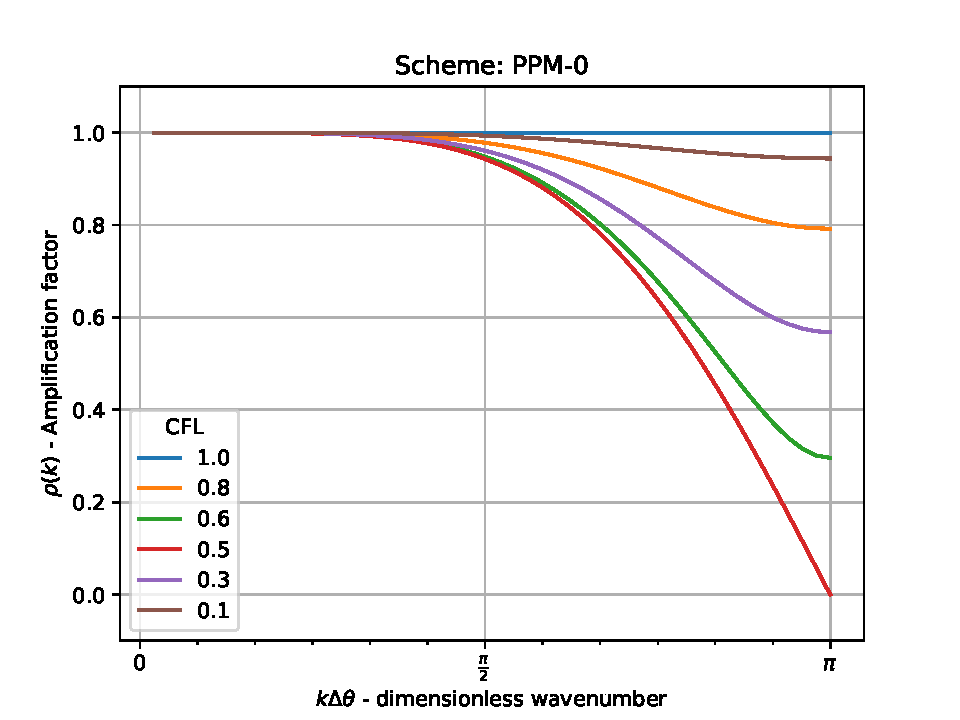
\includegraphics[width=0.49\linewidth]{stability_PPM-0}
	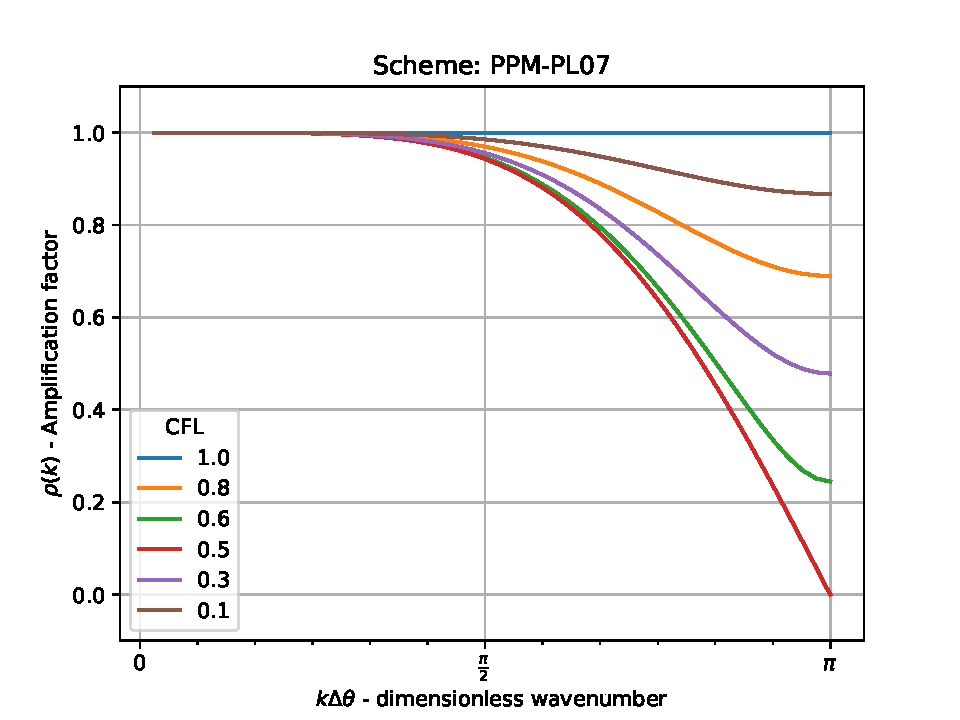
\includegraphics[width=0.49\linewidth]{stability_PPM-PL07}
	\caption{Amplification factor for the PPM (left) and hybrid PPM (right) schemes for different CFL numbers.}
	\label{chp2-fig-amplification}
\end{figure}
In order to investigate the consistency of the PPM scheme, we notice that when we are deducing the time average flux, 
we are making approximations of the form:
\begin{equation}
	\label{chp2-sec-flux:analysis-eq1}
	\int_{t^n}^{t^{n+1}} (uq)(x_{i+\frac{1}{2}},t) \,dt \approx
	\int_{x_{i+\frac{1}{2}}-\tilde{u}_{i+\frac{1}{2}}^n \Delta t}^{x_{i+\frac{1}{2}}}
	q_{PP}(x;Q^n)\,dx, 
\end{equation}
as we can see from Equations \eqref{chp-sec-flux:fL_1} and \eqref{chp-sec-flux:fR_1},
which basically replace $q$ by $q_{PP}$ and $X(t^n, t^{n+1},x_{i+\frac{1}{2}})$ by 
$x_{i+\frac{1}{2}}-\tilde{u}_{i+\frac{1}{2}}^n \Delta t$
on the right-hand side of Equation \eqref{chp2-sec-flux:approx1}.
As we shall see, the approximation \eqref{chp2-sec-flux:analysis-eq1}
has two sources of error: one related to the departure point estimation and another due to the
parabolic approximation.
The next Proposition \eqref{chp2-sec-flux:prop2} investigates how the departure point error
impacts on the approximation \eqref{chp2-sec-flux:analysis-eq1} replacing $q_{PP}$ by $q$.

\begin{prop}
	\label{chp2-sec-flux:prop2}
	Assume the framework of Problem \ref{chp2-sec2-prob2} with $q \in \mathcal{C}^1$  and $u \in \mathcal{C}^P$, for some $P\geq2$. 
	Furthermore, assume the CFL condition and that $\Delta x$ and $ \Delta t $ are small enough as in Proposition \ref{chp2-sec-flux:departurebound}.
	
	Assume also that for some time-average velocity $\tilde{u}^n_{i+\frac{1}{2}}$, we have
	$X(t^n,t^{n+1};x_{i+\frac{1}{2}}) = x_{i+\frac{1}{2}} - \tilde{u}^n_{i+\frac{1}{2}}\Delta t + C_{i+\frac{1}{2}}\Delta t^P$, 
	where the constants $C_{i+\frac{1}{2}}$ can be written as $C_{i+\frac{1}{2}} = F(\tilde{x}_{i+\frac{1}{2}}, \tilde{t}_{i+\frac{1}{2}})$ for 
	a $\mathcal{C}^1$ function $F:[a,b]^d \times [0,T]^d \to \mathbb{R}$ . 
	Besides that, assume $\tilde{x}_{i+\frac{1}{2}} \in [x_{i+\frac{1}{2}}-k\Delta x, x_{i+\frac{1}{2}} + k\Delta x]^d$, 
	where $k$ do not depend on $\Delta x$ and $\tilde{t}_{i+\frac{1}{2}} \in [t^n, t^{n+1}]^d$.
	Under all these assumptions, we have:
\begin{align*}
	&\bigg|\int_{t^n}^{t^{n+1}} (uq)(x_{i+\frac{1}{2}},s) \,ds 
	-\int^{x_{i+\frac{1}{2}}}_{x_{i+\frac{1}{2}}-\tilde{u}_{i+\frac{1}{2}}^n \Delta t} q(x,t^n)\,dx
	-\bigg( \int_{t^n}^{t^{n+1}} (uq)(x_{i-\frac{1}{2}},s) \,ds 
	-\int^{x_{i-\frac{1}{2}}}_{x_{i-\frac{1}{2}}-\tilde{u}_{i-\frac{1}{2}}^n \Delta t} q(x,t^n)\,dx  \bigg) \bigg| \\
	& \leq K_1 \Delta t^{P+1},
\end{align*}
	where $K_1$ depends on $q$ and $u$.
\end{prop}
\begin{proof}
	Using Equation \eqref{chp2-sec-flux:approx1} and the mean value theorem for integrals, we get: 
	\begin{align*}
	\label{chp-sec-flux:depint_5}
			  &\int_{t^n}^{t^{n+1}} (uq)(x_{i+\frac{1}{2}},s) \,ds 
			 -\int^{x_{i+\frac{1}{2}}}_{x_{i+\frac{1}{2}}-\tilde{u}_{i+\frac{1}{2}}^n \Delta t} q(x,t^n)\,dx =
			 \int^{x_{i+\frac{1}{2}}}_{X(t^n,t^{n+1};x_{i+\frac{1}{2}})} q(x,t^n)\,dx
			 -\int^{x_{i+\frac{1}{2}}}_{x_{i+\frac{1}{2}}-\tilde{u}_{i+\frac{1}{2}}^n \Delta t} q(x,t^n)\,dx \\ 
			 &= \int_{X(t^n,t^{n+1};x_{i+\frac{1}{2}})}^{x_{i+\frac{1}{2}}-\tilde{u}_{i+\frac{1}{2}}^n \Delta t} q(x,t^n)\,dx  
			 = \big(X(t^n,t^{n+1};x_{i+\frac{1}{2}}) - x_{i+\frac{1}{2}}+\tilde{u}_{i+\frac{1}{2}}^n \Delta t \big)
			 q(\mu_i,t^n) =  F(\tilde{x}_{i+\frac{1}{2}}, \tilde{t}_{i+\frac{1}{2}}) \Delta t^P q(\mu_{i+\frac{1}{2}},t^n),
	\end{align*}
	for some $\mu_{i+\frac{1}{2}} \in X_{i}\cup X_{i+1}$. Similarly, we have:
	\begin{align*}
	&\int_{t^n}^{t^{n+1}} (uq)(x_{i-\frac{1}{2}},s) \,ds 
	-\int^{x_{i-\frac{1}{2}}}_{x_{i-\frac{1}{2}}-\tilde{u}_{i-\frac{1}{2}}^n \Delta t} q(x,t^n)\,dx =
	F(\tilde{x}_{i-\frac{1}{2}},\tilde{t}_{i-\frac{1}{2}}) \Delta t^P q(\mu_{i-\frac{1}{2}},t^n),
	\end{align*}
and again, $\mu_{i-\frac{1}{2}} \in X_{i-1}\cup X_{i}$
We introduce the following auxiliary $\mathcal{C}^1$ function:
\begin{equation*}
	G(\nu) = F(\nu_1,\nu_2)q(\nu_3,t^n).
\end{equation*}
where $\nu =(\nu_1,\nu_2, \nu_3)$, $\nu_1 \in [a,b]^d$, $\nu_2 \in [0, T]^d$, $\nu_3 \in [a,b]$.
Introducing $\nu_{i+\frac{1}{2}} = (\tilde{x}_{i+\frac{1}{2}}, \tilde{t}_{i+\frac{1}{2}}, \mu_{i+\frac{1}{2}})$,
$\nu_{i-\frac{1}{2}} = (\tilde{x}_{i-\frac{1}{2}}, \tilde{t}_{i-\frac{1}{2}}, \mu_{i-\frac{1}{2}})$
and using the mean value theorem, we have:
\begin{align*}
	|G(\nu_{i+\frac{1}{2}})-G(\nu_{i-\frac{1}{2}})|  
	&\leq \bigg(\sup_{\nu \in [a,b]^d\times[0,T]^d\times[a,b]}{\|\nabla G(\nu) \|_{2d+1}} \bigg)\|\nu_{i+\frac{1}{2}}-\nu_{i-\frac{1}{2}}\|_{2d+1} \\
	&\leq \bigg(\sqrt{(d(2k+1)^2 + 9){\lambda^2}+d}\sup_{\nu \in [a,b]^d\times[0,T]^d\times[a,b]}{\|\nabla G(\nu) \|_{2d+1}} \bigg) \Delta t,
\end{align*}
where $\|\cdot\|_{D}$ is the 2-norm of $\mathbb{R}^{D}$ and we used that $\|\tilde{x}_{i+\frac{1}{2}}-\tilde{x}_{i-\frac{1}{2}}\|_{d}^2  \leq d(2k+1)^2\Delta x^2$, 
$|\tilde{\mu}_{i+\frac{1}{2}}-\tilde{\mu}_{i-\frac{1}{2}}| \leq 3 \Delta x$,
and $\|\tilde{t}_{i+\frac{1}{2}}-\tilde{t}_{i-\frac{1}{2}}\|_{d}^2 \leq d\Delta t^2$.
Finally, we have the desired bound:
\begin{align*}
	&\bigg|\int_{t^n}^{t^{n+1}} (uq)(x_{i+\frac{1}{2}},s) \,ds 
	-\int^{x_{i+\frac{1}{2}}}_{x_{i+\frac{1}{2}}-\tilde{u}_{i+\frac{1}{2}}^n \Delta t} q(x,t^n)\,dx
	-\bigg( \int_{t^n}^{t^{n+1}} (uq)(x_{i-\frac{1}{2}},s) \,ds 
	-\int^{x_{i-\frac{1}{2}}}_{x_{i-\frac{1}{2}}-\tilde{u}_{i-\frac{1}{2}}^n \Delta t} q(x,t^n)\,dx  \bigg) \bigg| \\
	&=|(G(\nu_{i+\frac{1}{2}})-G(\nu_{i-\frac{1}{2}}))|\Delta t^P \leq  K_1 \Delta t^{P+1},
\end{align*}
where $K_1 = \sqrt{(d(2k+1)^2 + 9){\lambda^2}+d}\sup_{\nu \in [a,b]^d\times[0,T]^d\times[a,b]}{\|\nabla G(\nu) \|_{2d+1}}$.
\end{proof}
\begin{remark}
If the departure point is computed using Equation \eqref{chp-sec-flux:departurepoint3}, it follows from Proposition \ref{chp-sec-flux:dp_euler}
that $P=2$, $k=3$, $d=2$.
The function $F$ is defined by the right-hand side of Equation \eqref{chp-sec-flux:departurepoint6}.
\end{remark}
The next proposition gives a measure of the impact of the Piecewise-Parabolic approximation
on the time average flux, considering this last computed using an estimated departure point.
\begin{prop}
	\label{chp2-sec-flux:prop3}
	Assume the framework of Problem \ref{chp2-sec2-prob2}.
	If $q \in \mathcal{C}^5$ and $u \in \mathcal{C}^1$, then:
	\begin{align*}
	 &\bigg|
	\frac{1}{\Delta t}\int^{x_{i+\frac{1}{2}}}_{x_{i+\frac{1}{2}}-\tilde{u}_{i+\frac{1}{2}}^n \Delta t} q(x,t^n)\,dx -
	\mathcal{F}(Q(t_n)(\mathcal{S}_{i+\frac{1}{2}}),\tilde{u}^n_{i+\frac{1}{2}}) 
	-\bigg(\frac{1}{\Delta t}\int^{x_{i-\frac{1}{2}}}_{x_{i-\frac{1}{2}}-\tilde{u}_{i-\frac{1}{2}}^n \Delta t} q(x,t^n)\,dx -
	\mathcal{F}(Q(t_n)\mathcal{S}_{i-\frac{1}{2}},\tilde{u}^n_{i-\frac{1}{2}})\bigg) \bigg|\\
	&\leq K_2\Delta x^4,
	\end{align*}
	where $K_2$ depends on $q$ and $u$.
\end{prop}
\begin{proof}
	We denote by $q_{PP}$ the piecewise-parabolic approximation of $Q(t^n)$. Then:
	\begin{equation*}
	\frac{1}{\Delta t}\int^{x_{i+\frac{1}{2}}}_{x_{i+\frac{1}{2}}-\tilde{u}_{i+\frac{1}{2}}^n \Delta t} q(x,t^n)\,dx -
	\mathcal{F}(Q(t_n)(\mathcal{S}_{i+\frac{1}{2}}),\tilde{u}^n_{i+\frac{1}{2}}) = 	
	\frac{1}{\Delta t}\int^{x_{i+\frac{1}{2}}}_{x_{i+\frac{1}{2}}-\tilde{u}_{i+\frac{1}{2}}^n \Delta t} q(x,t^n)\,dx -
	\frac{1}{\Delta t}\int^{x_{i+\frac{1}{2}}}_{x_{i+\frac{1}{2}}-\tilde{u}_{i+\frac{1}{2}}^n \Delta t} q_{PP}(x;Q(t^n))\,dx
	\end{equation*}
	and
	\begin{equation*}
	\frac{1}{\Delta t}\int^{x_{i-\frac{1}{2}}}_{x_{i-\frac{1}{2}}-\tilde{u}_{i-\frac{1}{2}}^n \Delta t} q(x,t^n)\,dx -
	\mathcal{F}(Q(t_n)(\mathcal{S}_{i-\frac{1}{2}}),\tilde{u}^n_{i-\frac{1}{2}}) = 	
	\frac{1}{\Delta t}\int^{x_{i-\frac{1}{2}}}_{x_{i-\frac{1}{2}}-\tilde{u}_{i-\frac{1}{2}}^n \Delta t} q(x,t^n)\,dx -
	\frac{1}{\Delta t}\int^{x_{i-\frac{1}{2}}}_{x_{i-\frac{1}{2}}-\tilde{u}_{i-\frac{1}{2}}^n \Delta t} q_{PP}(x;Q(t^n))\,dx.
\end{equation*}
	Similarly to Proposition \ref{prop:ppm-bound4}, we can write:
	\begin{align*}
		q(x,t^n)-q_{PP}(x;Q(t^n)) = &C_1(\mu_1, \mu_2) \Delta x ^4 + C_2(\mu_3, \mu_4) \Delta x ^2(x-x_L)
		+ \frac{C_3}{2}(\mu_5, \mu_6)\Delta x (x-x_L)^2  \\&+C_4(\mu_7)(x-x_L)^3,
	\end{align*}
	where $C_1, C_2$, $C_3$ and $C_4$ are given by Equations \eqref{prop:ppm-bound1-eq3},
	\eqref{prop:ppm-bound2-eq2}, \eqref{prop:ppm-bound3-eq2} and \eqref{prop:ppm-bound4-eq3} respectively,
	$x_L$ is the left boundary of the control volume that contains $x$ ($X_i$ or $X_{i+1}$) and 
	$\mu_k \in [x_{i+\frac{1}{2}} - 3\Delta x,x_{i+\frac{1}{2}} + 3\Delta x]$, $\forall k =1, \cdots, 7$.
	Similarly to Proposition \ref{chp2-sec-flux:prop2}, using the mean value theorem for integrals, one can write:
	\begin{equation}
	\label{chp2-sec-flux:prop3-eq1}
	\int^{x_{i+\frac{1}{2}}}_{x_{i+\frac{1}{2}}-\tilde{u}_{i+\frac{1}{2}}^n \Delta t} (q(x,t^n)-q_{PP}(x;Q(t^n)))\,dx
	= F(\mu^1)\Delta x^4,
	\end{equation}
	and
	\begin{equation}
	\label{chp2-sec-flux:prop3-eq2}
	\int^{x_{i-\frac{1}{2}}}_{x_{i-\frac{1}{2}}-\tilde{u}_{i-\frac{1}{2}}^n \Delta t} (q(x,t^n)-q_{PP}(x;Q(t^n)))\,dx
	= F(\mu^2)\Delta x^4,
	\end{equation}
	for an auxiliary function $F:[a,b]^8 \to \mathbb{R}$, $F\in\mathcal{C}^1$, where $F$ depends on $q$, $u$,
	and $C_1, C_2, C_3$ and $C_4$. Subtracting Equation \eqref{chp2-sec-flux:prop3-eq2} from Equation \eqref{chp2-sec-flux:prop3-eq1}
	and using the mean value theorem, we get the desired inequality.
	\end{proof}
Now we are able to tackle the consistency problem on the next proposition.
\begin{prop}
	\label{chp2-sec-flux:prop4}
	Assume the same hypothesis of Proposition \ref{chp2-sec-flux:prop2} and Proposition \ref{chp2-sec-flux:prop3}.
	Denote by $q_{PP}$ the Piecewise-Parabolic approximation of $q(x,t^n)$. Then, the LTE given by Equation
	\eqref{consistency-1d-eq2} satisfies:
	\begin{equation}
		|\tau_i^n|\leq M_1 \Delta t^{P-1} + M_2\Delta x^3,
	\end{equation}
	where $M_1$ and $M_2$ are constants depending only on $q$ and $u$.
\end{prop}
\begin{proof}
	We have:
	\begin{align*}
	 &\Delta x  \tau_i^n = \bigg|
	 \frac{1}{\Delta t}\int_{t^n}^{t^{n+1}} (uq)(x_{i+\frac{1}{2}},s) \,ds - 
	 \mathcal{F}(Q(t_n)(\mathcal{S}_{i+\frac{1}{2}}),\tilde{u}^n_{i+\frac{1}{2}})
	 - \frac{1}{\Delta t}\int_{t^n}^{t^{n+1}} (uq)(x_{i-\frac{1}{2}},s) \,ds +
	 \mathcal{F}(Q(t_n)(\mathcal{S}_{i-\frac{1}{2}}),\tilde{u}^n_{i-\frac{1}{2}}) \bigg| = \\
	 & \frac{1}{\Delta t} \bigg|
	 \int_{t^n}^{t^{n+1}} (uq)(x_{i+\frac{1}{2}},s) \,ds - 
	 \int^{x_{i+\frac{1}{2}}}_{x_{i+\frac{1}{2}}-\tilde{u}_{i+\frac{1}{2}}^n \Delta t} q_{PP}(x)\,dx
	 -\bigg(\int_{t^n}^{t^{n+1}} (uq)(x_{i-\frac{1}{2}},s) \,ds - 
	 \int^{x_{i-\frac{1}{2}}}_{x_{i-\frac{1}{2}}-\tilde{u}_{i-\frac{1}{2}}^n \Delta t} q_{PP}(x)\,dx  
	  \bigg)\bigg| =\\
	 &\frac{1}{\Delta t} \bigg|
	 \int_{t^n}^{t^{n+1}} (uq)(x_{i+\frac{1}{2}},s) \,ds 
	-\int^{x_{i+\frac{1}{2}}}_{x_{i+\frac{1}{2}}-\tilde{u}_{i+\frac{1}{2}}^n \Delta t} q(x,t^n)\,dx 
	+\int^{x_{i+\frac{1}{2}}}_{x_{i+\frac{1}{2}}-\tilde{u}_{i+\frac{1}{2}}^n \Delta t} q(x,t^n)\,dx 
	-\int^{x_{i+\frac{1}{2}}}_{x_{i+\frac{1}{2}}-\tilde{u}_{i+\frac{1}{2}}^n \Delta t} q_{PP}(x)\,dx \\
	 &-\bigg(\int_{t^n}^{t^{n+1}} (uq)(x_{i-\frac{1}{2}},s) \,ds 
	-\int^{x_{i-\frac{1}{2}}}_{x_{i-\frac{1}{2}}-\tilde{u}_{i-\frac{1}{2}}^n \Delta t} q(x,t^n)\,dx 
	+\int^{x_{i-\frac{1}{2}}}_{x_{i-\frac{1}{2}}-\tilde{u}_{i-\frac{1}{2}}^n \Delta t} q(x,t^n)\,dx 
	-\int^{x_{i-\frac{1}{2}}}_{x_{i-\frac{1}{2}}-\tilde{u}_{i-\frac{1}{2}}^n \Delta t} q_{PP}(x)\,dx 
	 \bigg) \bigg| \leq \\
	 &\frac{1}{\Delta t} \bigg|
	\int_{t^n}^{t^{n+1}} (uq)(x_{i+\frac{1}{2}},s) \,ds 
	-\int^{x_{i+\frac{1}{2}}}_{x_{i+\frac{1}{2}}-\tilde{u}_{i+\frac{1}{2}}^n \Delta t} q(x,t^n)\,dx 
	-\bigg(\int_{t^n}^{t^{n+1}} (uq)(x_{i-\frac{1}{2}},s) \,ds 
	-\int^{x_{i-\frac{1}{2}}}_{x_{i-\frac{1}{2}}-\tilde{u}_{i-\frac{1}{2}}^n \Delta t} q(x,t^n)\,dx \bigg)\bigg|+\\
     &\frac{1}{\Delta t}\bigg| 
	 \int^{x_{i+\frac{1}{2}}}_{x_{i+\frac{1}{2}}-\tilde{u}_{i+\frac{1}{2}}^n \Delta t} q(x,t^n)\,dx 
	-\int^{x_{i+\frac{1}{2}}}_{x_{i+\frac{1}{2}}-\tilde{u}_{i+\frac{1}{2}}^n \Delta t} q_{PP}(x) \,dx 
	-\bigg(\int^{x_{i-\frac{1}{2}}}_{x_{i-\frac{1}{2}}-\tilde{u}_{i-\frac{1}{2}}^n \Delta t} q(x,t^n)\,dx 
	-\int^{x_{i-\frac{1}{2}}}_{x_{i-\frac{1}{2}}-\tilde{u}_{i-\frac{1}{2}}^n \Delta t} q_{PP}(x) \,dx 
	\bigg) \bigg| 
	\end{align*}
	Therefore, it follows from Propositions \ref{chp2-sec-flux:prop2} and \ref{chp2-sec-flux:prop3} that
	\begin{align*}
		|\tau_i^n| \leq \frac{1}{\Delta x \Delta t} K_1 \Delta t^{P+1} + \frac{1}{\Delta x} K_2 \Delta x^4 = 
		K_1 \lambda \Delta t^{P-1} + K_2 \Delta x^3,
	\end{align*}
	from which the proposition follows.
\end{proof}

	Thus, it follows from Proposition \ref{chp2-sec-flux:prop3} that the PPM scheme is consistent in the $\infty$-norm
	and has two sources of error: one related to the departure point calculation and another due to the parabolic approximation.
	In particular, the PPM flux using the departure point from Equation \eqref{chp-sec-flux:departurepoint3}, 
	we have a first-order error related to the departure point computation. 
	We point out that, if the velocity is constant, then no error is obtained
	using the PPM flux, except for the approximation $q_{PP}$ to $q$.
\newpage
\section{Numerical experiments}
\label{chp2-sec-numerical-exp}
This Section is dedicated to presenting the numerical results of the PPM and its variations discussed here.
For non-monotonic schemes, we are going to consider
the original PPM from \citet{colella:1984}(hereafter will be referred as \textbf{PPM-0}) and 
the hybrid PPM from \citet{putman:2007} (hereafter \textbf{PPM-PL07}).
For monotonic schemes, we are going to consider the monotonization schemes from 
\citet{colella:1984}  (hereafter \textbf{PPM-CW84}) and \citet{lin:2004} (hereafter \textbf{PPM-L04}), which are referred to as CW84 monotonization 
and L04 monotonization hereafter.
In Subsection \ref{chp2-sec-numerical-exp-1} we present results 
using the linear advection equation with constant velocity
and in Subsection \ref{chp2-sec-numerical-exp-2}
the results are based on the linear advection equation with variable velocity.
The code used in this Section may be found in Appendix \ref{anexo-code}.

Inspired by \citet{trefethen:2000}, we also consider the following periodic Gaussian profile:
\begin{equation}
	\label{chp2-ic2}
	q(x) = \exp(-10\cos^2 (2\pi x)),\quad x \in [0,1].
\end{equation}
For the linear advection equation with constant velocity we shall adopt the $u=0.2$ and 
a CFL number equal to $0.8$.
The spatial domain will be given by $[0,1]$ and the time integration interval will be $[0,5]$. 
We again use $\Delta x^{(k)}-$grids with $\Delta x^{(k)} = 1/2^k$ for $k=4,\ldots, 10$.
Since we are going to assume periodic boundary conditions, the period is equal to $5$. 
Hence, the simulations presented here shall advect an initial profile for one time period. 
The departure schemes RK1 and RK2 introduced in Section \ref{chp2-sec-flux} compute
the departure point exactly in this case, therefore we are going only to use the RK1 scheme.
This shall be the general setup for all simulations presented in this subsection. 
What will distinguish the simulations is the initial condition.
We consider $q_0$ given by Equations \eqref{chp2-ic1} and \eqref{chp2-ic2} as
in Subsection \ref{chp2-sec-numerical-exp-1}.
We also consider a discontinuous initial condition given by:
\begin{equation}
	\label{chp2-ic3}
		q_0(x) =  
  \begin{cases}
		1 & \text{if } x \in [0.4,0.6],\\
		0 & \text{otherwise}.
  \end{cases}
\end{equation}
It is easy to check that the  exact solution of Problem \ref{chp2-sec2-prob1}
is given by $q_0(x-ut)$ for all $q_0$ presented here. We are going to consider the relative
error in the maximum norm:
\begin{equation*}
	E_k = \max_{n=0,\cdots, N_T}
	\frac{\| Q^n - Q(t^n) \|_{\infty, \Delta x}}{\|Q(t^n)\|_{\infty, \Delta x}}.
\end{equation*}
The convergence rate is defined by
\begin{equation*}
	CR_k = \frac{\ln{\bigg(\frac{E_{k}}{E_{k-1}}}\bigg)}{\ln 2}, \quad \text{for} \quad k = 5, \cdots 10.
\end{equation*}
As pointed in Subsection \ref{chp2-num-exp-recon}, when $q_0$ is given by Equation \eqref{chp2-ic2},
we are going to compute the initial average values $Q_i(0)$ using
the initial values of $q^0_i$ at the control volume centroids, which is second-order 
accurate by Proposition \ref{prop-bound-centroid}. 
In the error calculation, only when $q_0$ is given by Equation \eqref{chp2-ic2},
we replace $Q_{i}(t^n)$ by its centroid value $q_{i}(t^n)$, which again gives
a second-order approximation by Proposition \ref{prop-bound-centroid}.
Therefore, since $q_0$ is smooth, we expect that the error convergence shall be at least second-order accurate. The relative change at time-step $n$ in the mass is computed as 
\begin{equation*}
	\frac{|M^n-M^0|}{|M_0|},
\end{equation*}
where $M^n$ is given by Equation \eqref{1d-fv-mass}. For all the simulations, the
mass is preserved with machine precision. 

When $q_0$ is given by Equation \eqref{chp2-ic3}, it follows from Figure
\ref{chp2-sec-exp-adv1} that monotonic scheme PPM-L04 is less dissipative than PPM-CW84,
and PPM-L07 is less dissipative than PPM-0, which agrees with the amplification factors
from Figure \ref{chp2-fig-amplification}.
This may be noticed when we compare the extreme values. 
Furthermore, both monotonic schemes avoid negative values.
For the Gaussian wave, we make similar conclusions from Figure \ref{chp2-sec-exp-adv2}.
The order of convergence of the PPM-0 and PPM-PL07 are equal to three as expected 
(Figure \ref{chp2-sec-exp-adv1-2}) for $q_0$ from Equation \eqref{chp2-ic3}.
Notice that, even though the initial average of the  Gaussian profile is computed with a
second-order approximation, the final error is third-order accurate as shown in Figure
\ref{chp2-sec-exp-adv2-2}. In all cases, the convergence order of the monotonic schemes
is approximately 1.5 and this order reduction is expected by Godunov's theorem. 
The major advantage of the monotonic schemes is observed in Figure \ref{chp2-sec-exp-adv3},
where we observe that the monotonic schemes prevent all the strong oscillations
presented in the non-monotonic schemes, and they avoid generation of new extrema as well.
\begin{figure}[!htb]
  \centering
  \begin{subfigure}{0.49\textwidth}
    \centering
			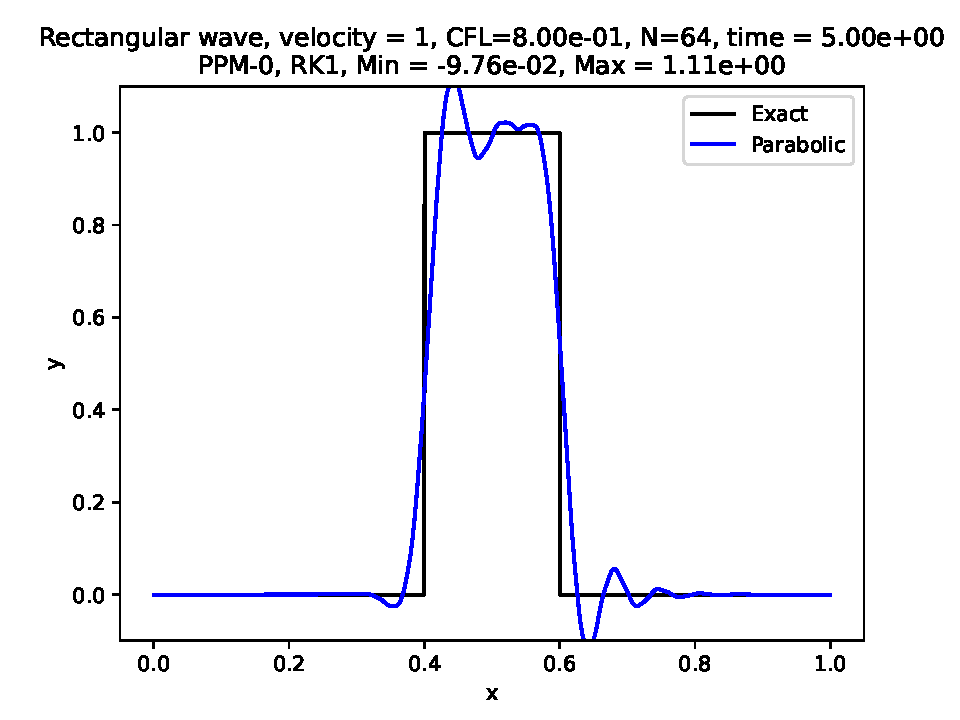
\includegraphics[width=1\linewidth]{1d_adv_tc2_ic4_vf1_t79_N64_PPM-0_dpRK1}
			\caption{PPM-0.\label{chp2-sec-exp-adv3-a}}
  \end{subfigure}
  \begin{subfigure}{0.49\textwidth}
    \centering
			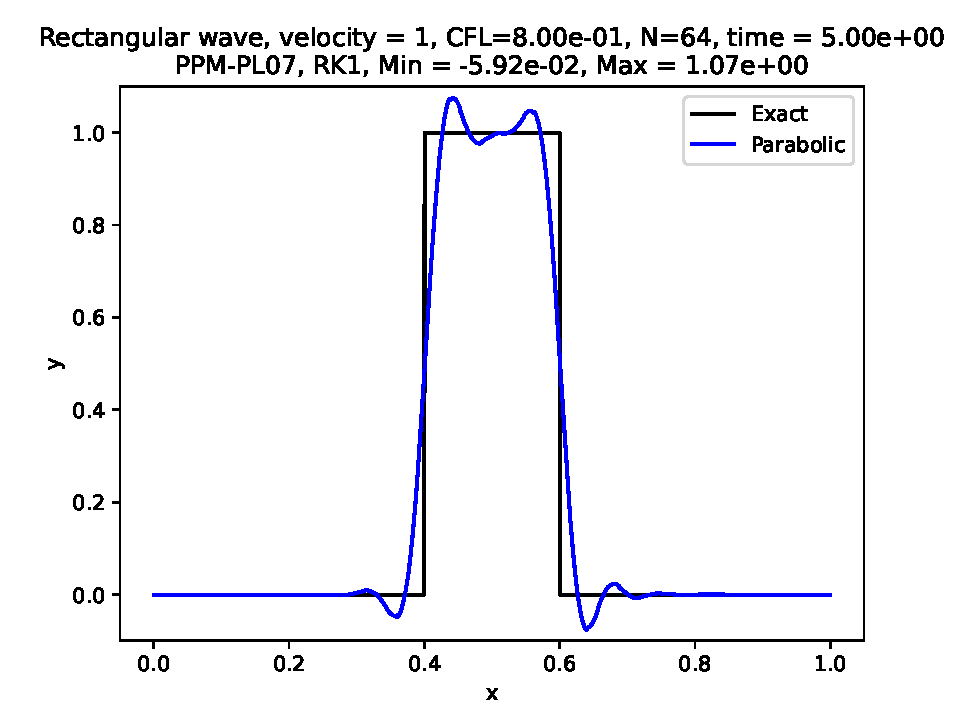
\includegraphics[width=1\linewidth]{1d_adv_tc2_ic4_vf1_t79_N64_PPM-PL07_dpRK1}
			\caption{PPM-PL07.\label{chp2-sec-exp-adv3-b}}
  \end{subfigure}

  \begin{subfigure}{0.49\textwidth}
    \centering
		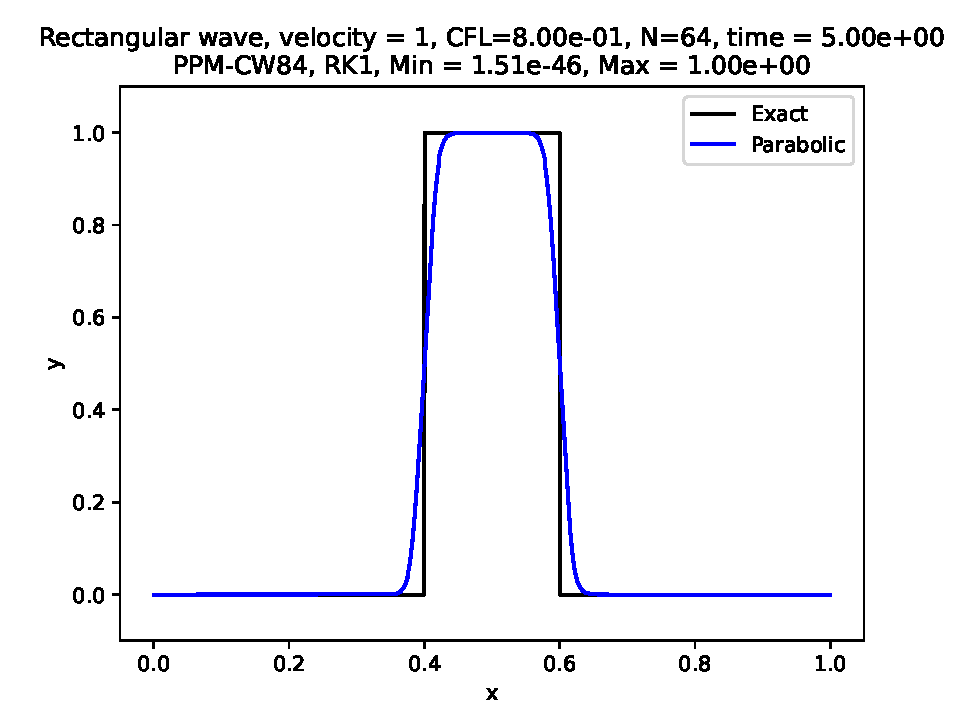
\includegraphics[width=1\linewidth]{1d_adv_tc2_ic4_vf1_t79_N64_PPM-CW84_dpRK1}
    \caption{PPM-CW84.\label{chp2-sec-exp-adv3-c}}
  \end{subfigure}
  \begin{subfigure}{0.49\textwidth}
    \centering
			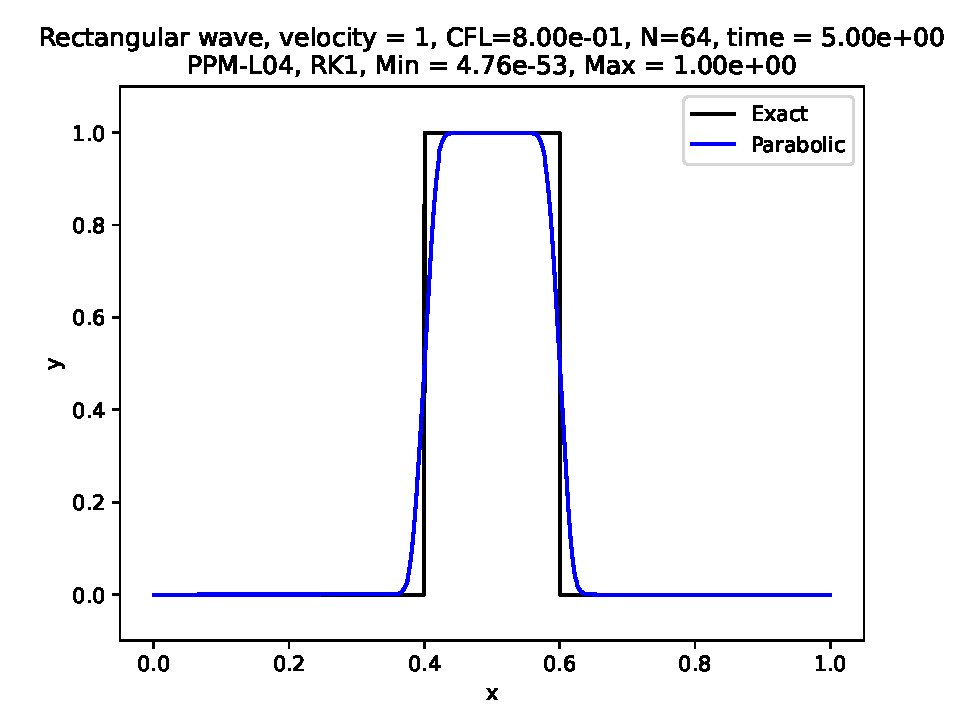
\includegraphics[width=1\linewidth]{1d_adv_tc2_ic4_vf1_t79_N64_PPM-L04_dpRK1}
      \caption{PPM-L04.\label{chp2-sec-exp-adv3-d}}
  \end{subfigure} 
	\caption{Linear advection experiment using a constant velocity equal to $0.1$,
		a CFL number equal to $0.8$, $N=32$ cells, and the initial condition is given by Equation \eqref{chp2-ic3}.
		These figures show the advected profile after 5 time units (one time period).
		Reconstruction schemes employed: PPM-0 (a), PPM-PL07 (b), PPM-CW84
		(c) and PPM-L04 (d).\label{chp2-sec-exp-adv3}}
\end{figure}

In this Subsection, we shall investigate the how the PPM schemes behave when the velocity
is variable. The initial condition is given by Equation \eqref{chp2-ic2}.
The relative errors are computed using the centroid values of $q$ as described in
Section \ref{chp2-sec-numerical-exp-2}. 
We are going to consider the velocity
\begin{equation}
	\label{chp2-vel2}
	u(x,t) = u_0\cos{\bigg(\frac{\pi t}{T}\bigg)}\sin^2\bigg(\pi \bigg(x-\frac{t}{T}\bigg)\bigg) + u_1.
\end{equation}
We adopt the parameters $u_0 = u_1 = 0.2$,  and $T = 5$.
In this case, the solution has a period equal to 5, then the profile returns to its
initial shape and position after 5 time units we can compute the error.
We point out that the velocity from Equation \eqref{chp2-vel2} is based on the deformational
flow test case from on \citet{nair:2010}. Since the velocity is variable, we are going to
use the departure point schemes RK1 and RK2 described in Section \ref{chp2-sec-flux}.

\begin{figure}[!htb]
  \centering
  \begin{subfigure}{0.49\textwidth}
    \centering
			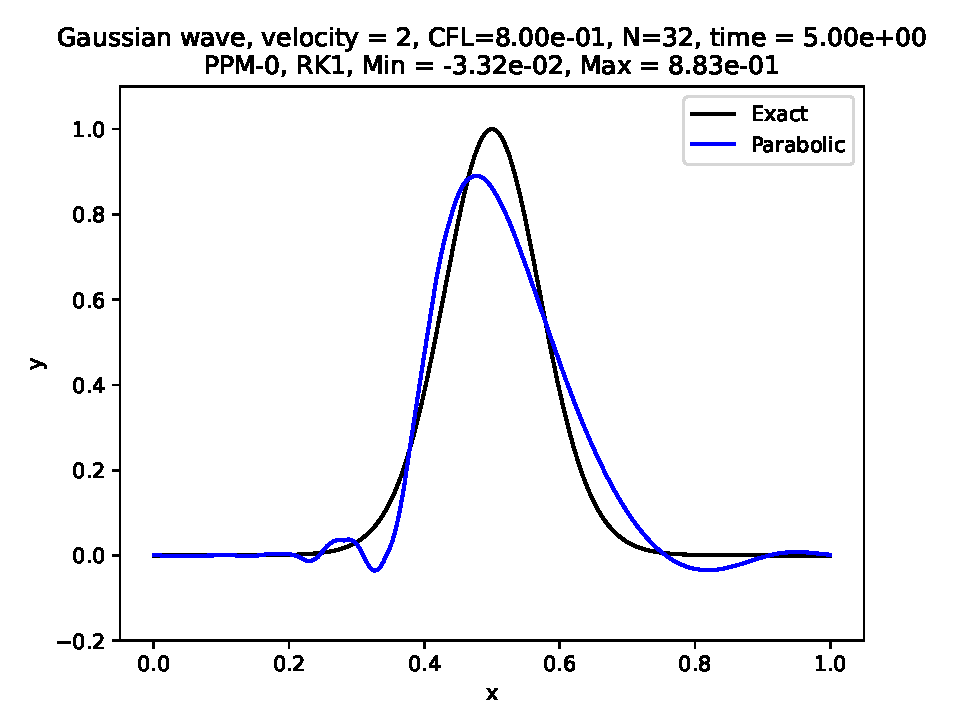
\includegraphics[width=1\linewidth]{1d_adv_tc1_ic2_vf2_t79_N32_PPM-0_dpRK1}
			\caption{PPM-0.\label{chp2-sec-exp-adv6-a}}
  \end{subfigure}
  \begin{subfigure}{0.49\textwidth}
    \centering
			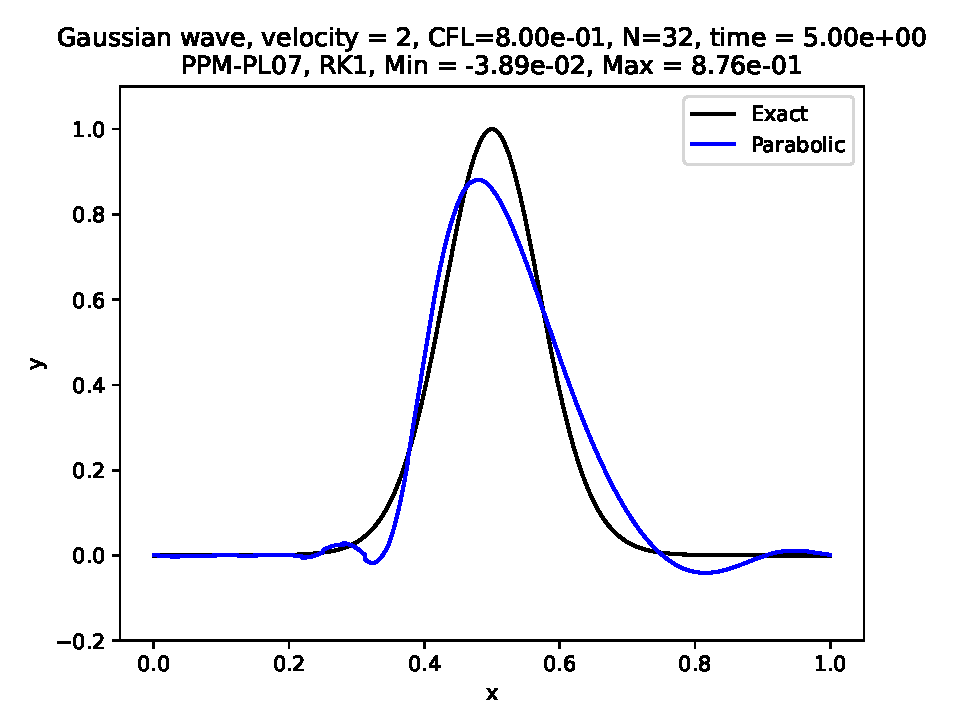
\includegraphics[width=1\linewidth]{1d_adv_tc1_ic2_vf2_t79_N32_PPM-PL07_dpRK1}
			\caption{PPM-PL07.\label{chp2-sec-exp-adv6-b}}
  \end{subfigure}

  \begin{subfigure}{0.49\textwidth}
    \centering
		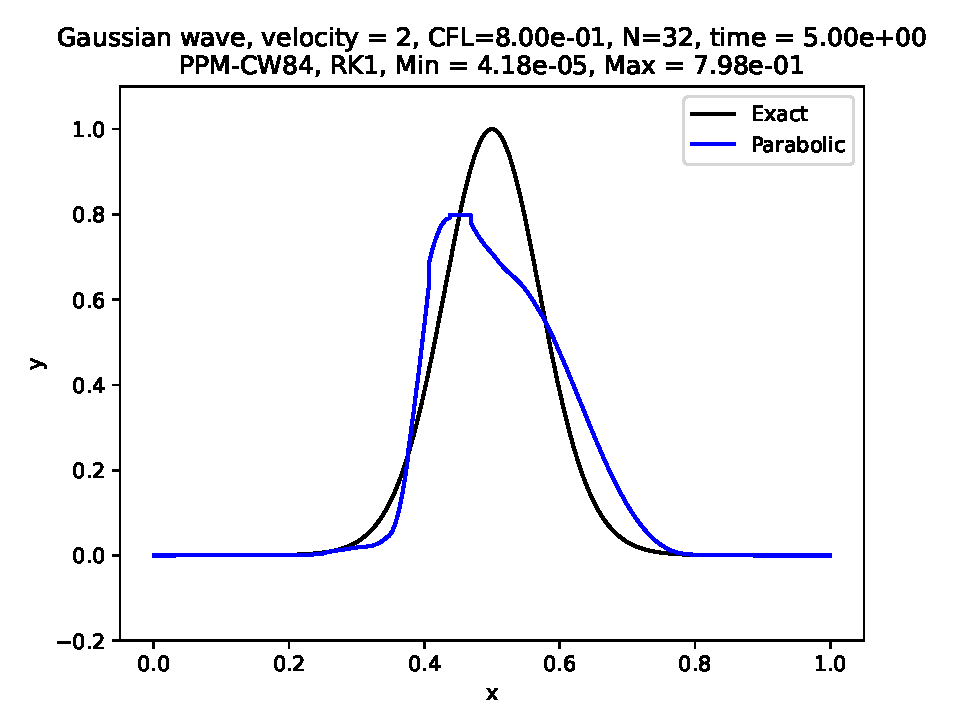
\includegraphics[width=1\linewidth]{1d_adv_tc1_ic2_vf2_t79_N32_PPM-CW84_dpRK1}
    \caption{PPM-CW84.\label{chp2-sec-exp-adv6-c}}
  \end{subfigure}
  \begin{subfigure}{0.49\textwidth}
    \centering
			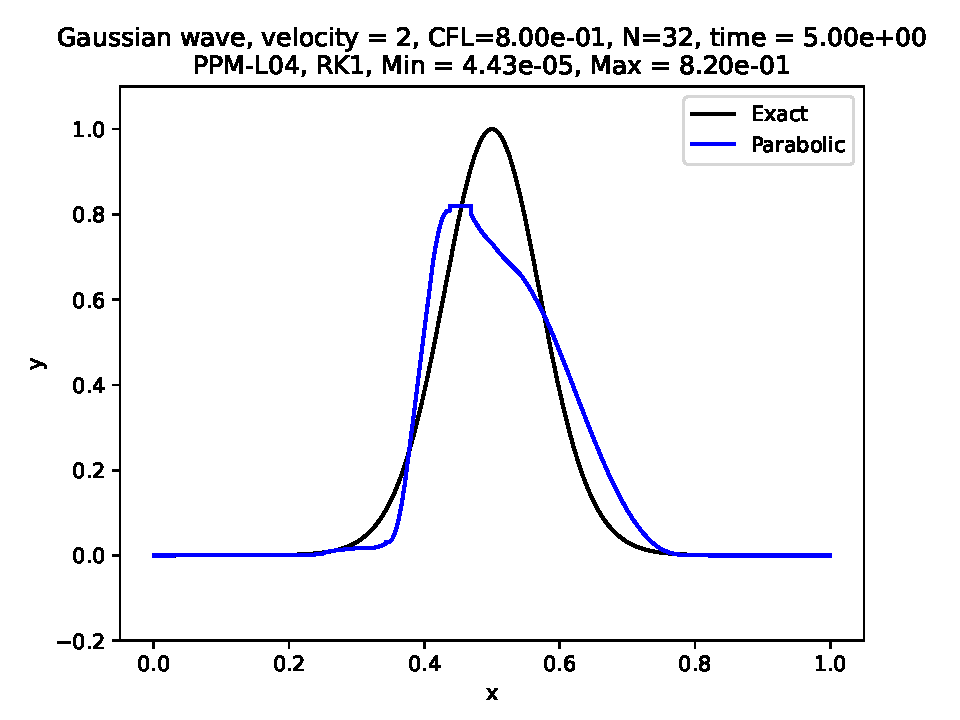
\includegraphics[width=1\linewidth]{1d_adv_tc1_ic2_vf2_t79_N32_PPM-L04_dpRK1}
      \caption{PPM-L04.\label{chp2-sec-exp-adv6-d}}
  \end{subfigure} 
	\caption{ 
		Similar to Figure \ref{chp2-sec-exp-adv1} but using $N=32$, 
	the initial condition given by Equation \eqref{chp2-ic2} and the variable velocity given by Equation
	\eqref{chp2-vel2} \label{chp2-sec-exp-adv6}.}
\end{figure}
In Figure \ref{chp2-sec-exp-adv5} we show the numerical after half period using the RK1
scheme and $N=32$. 
We also depict a reference solution in Figure \ref{chp2-sec-exp-adv5-e} at a high resolution
($N=1024$).
In Figure \ref{chp2-sec-exp-adv6} we show the profile obtained for each PPM scheme after
one period.
From Figures \ref{chp2-sec-exp-adv5} and \ref{chp2-sec-exp-adv6} we get a similar
conclusion about the dissipation of each scheme as in Section \ref{chp2-sec-numerical-exp-2}.
The difference between the schemes RK1 and RK2 is clear when we observe the relative error
in Figure \ref{chp2-sec-exp-adv6-2} and the convergence rate in
Figure \ref{chp2-sec-exp-adv6-3}.
The RK1 scheme leads to a first-order in the departure point that dominates the total error
for all PPM schemes, in agreement with Proposition \ref{chp2-sec-flux:prop4}.
When we employ the RK2 scheme, we can achieve third-order for the schemes PPM-0
and PPM-L07 which is better than the expected from Proposition \ref{chp2-sec-flux:prop4}.
This experiment illustrates the impact of the error in the departure point calculation
in the total error.

\begin{figure}[!htb]
  \centering
  \begin{subfigure}{0.49\textwidth}
    \centering
		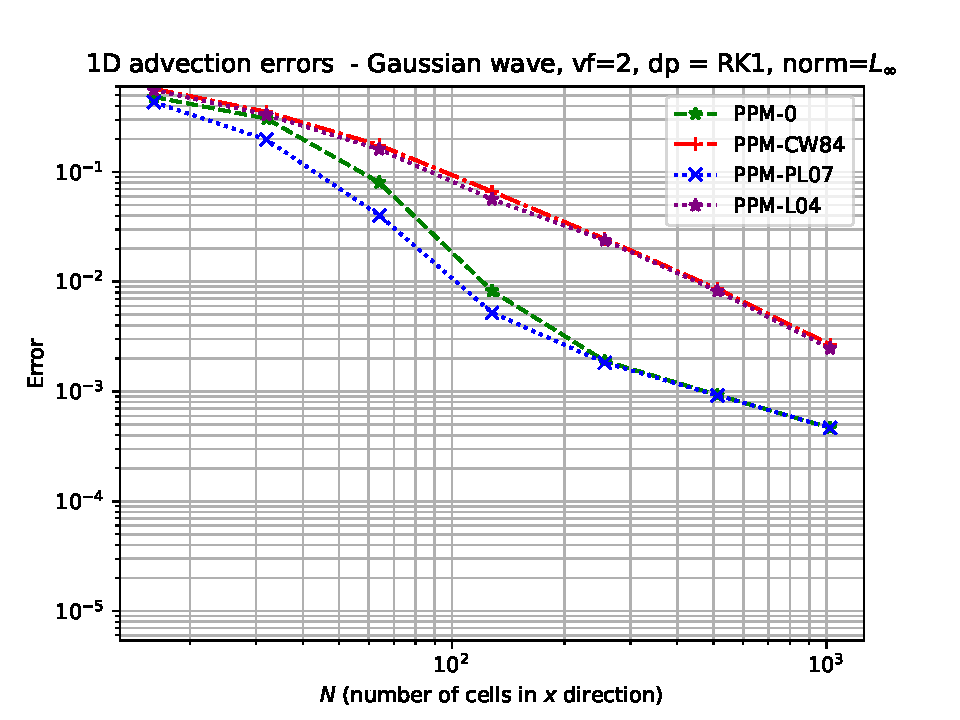
\includegraphics[width=1\linewidth]{1d_adv_tc2_ic2_vf2_dpRK1_normlinf_parabola_errors}
		\caption{RK1.\label{chp2-sec-exp-adv6-error-rk1}}
  \end{subfigure}
  \begin{subfigure}{0.49\textwidth}
    \centering
			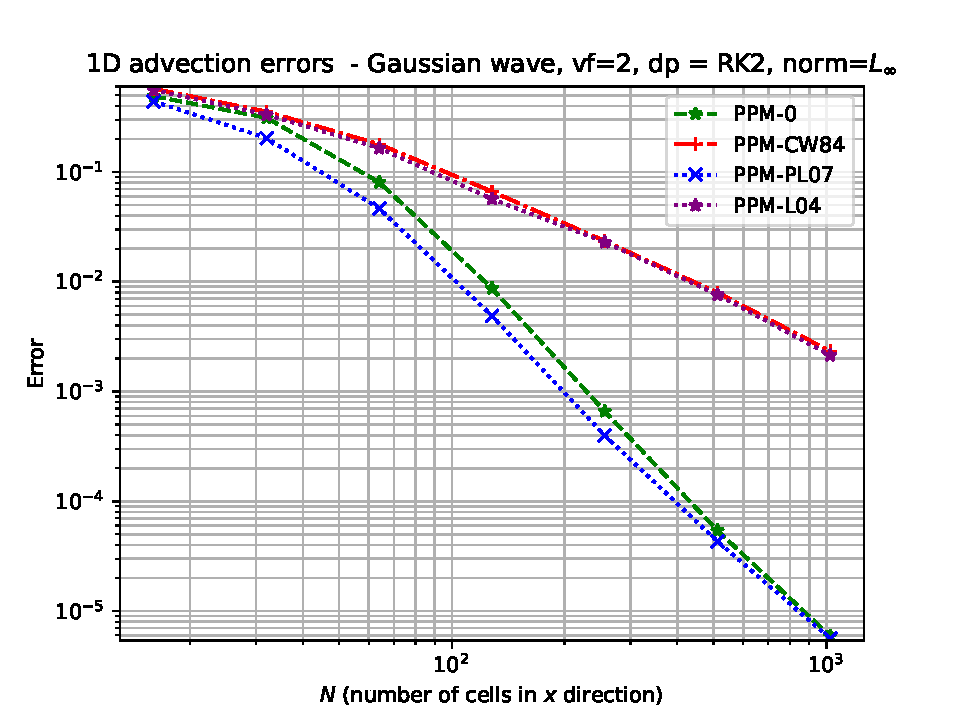
\includegraphics[width=1\linewidth]{1d_adv_tc2_ic2_vf2_dpRK2_normlinf_parabola_errors}
		\caption{RK2.\label{chp2-sec-exp-adv6-rl3}}
  \end{subfigure}
	\caption{Relative error for different PPM schemes using the RK1 (left) and RK2 (right)
	departure point scheme for the initial condition given by Equation
	\eqref{chp2-ic2} and the variable 
	velocity given by Equation \eqref{chp2-vel2}.\label{chp2-sec-exp-adv6-2}}
\end{figure}

\begin{figure}[!htb]
	\centering
	\begin{subfigure}{0.49\textwidth}
		\centering
		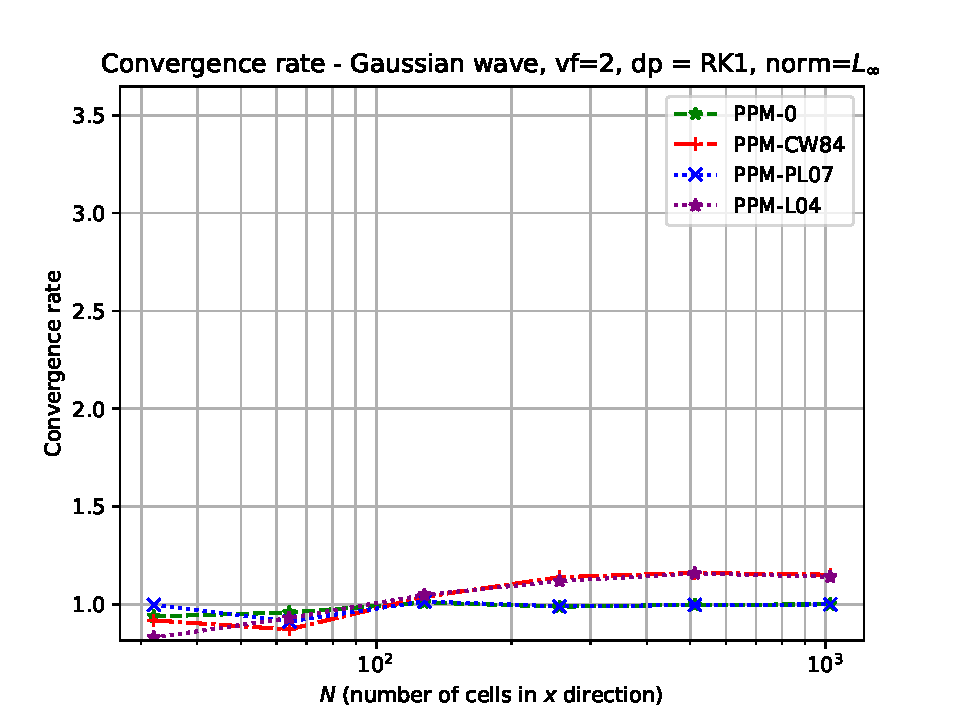
\includegraphics[width=1\linewidth]{1d_adv_tc2_ic2_vf2_dpRK1_normlinf_convergence_rate}
		\caption{RK1.\label{chp2-sec-exp-adv6-cr-rk1}}
	\end{subfigure}
	\begin{subfigure}{0.49\textwidth}
		\centering
		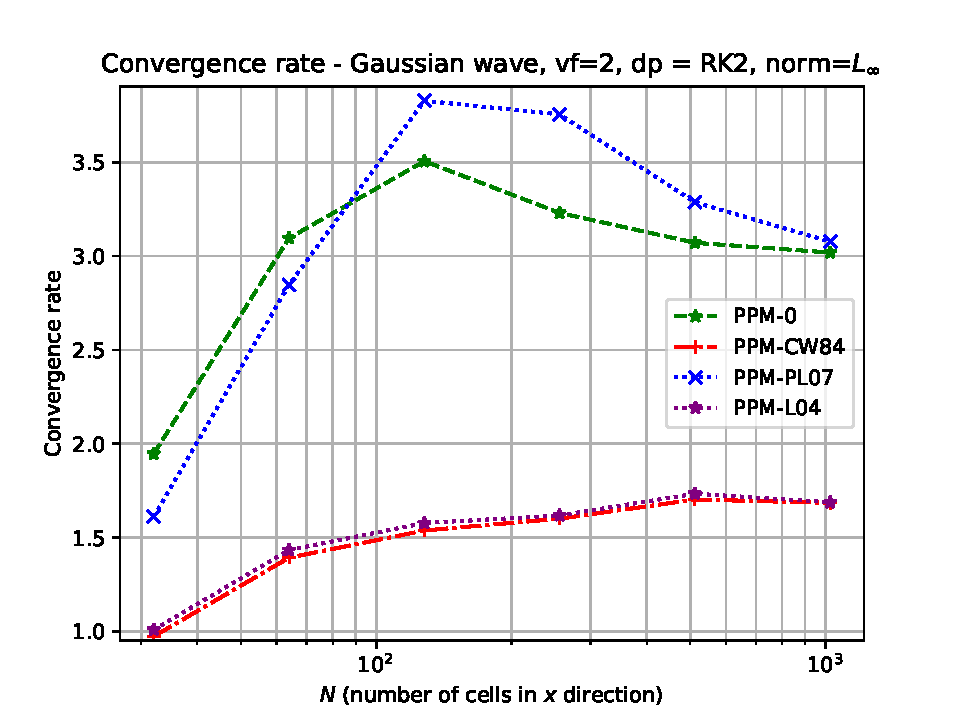
\includegraphics[width=1\linewidth]{1d_adv_tc2_ic2_vf2_dpRK2_normlinf_convergence_rate}
		\caption{RK2.\label{chp2-sec-exp-adv6-cf-RK2}}
	\end{subfigure}
	\caption{Convergence rate for different PPM schemes using the RK1 (left) and RK2 (right)
	departure point scheme for the initial condition given by Equation
	\eqref{chp2-ic2} and the variable 
	velocity given by Equation \eqref{chp2-vel2}.\label{chp2-sec-exp-adv6-3}}
\end{figure}

\section{Concluding remarks}
\label{chp2-sec-conclusion}
In this Chapter, we gave a general overview of 1D finite-volume schemes for the
advection equation. We saw that 1D-FV schemes require two tasks. 
The first task is to reconstruct a function from its average values. 
The second task is to compute the departure point of the control volume edges.
Each task introduces an error in the consistency error, impacting the final error, 
as we have shown theoretically.
The first task was performed using the PPM from \citet{colella:1984} 
and some of its variants. Without monotonicity constraints, we were able to 
achieve third in the reconstruction process.
The second task was performed using the first-order departure point calculation from
\citet{colella:1984} (RK1). We also explored a third-order approach using a three stages
Runge-Kutta scheme (RK2) to integrate the departure point ODE.

From the numerical experiments, we observe that the PPM-L07 \citep{putman:2007},
which uses a fifth-order reconstruction at the edges, leads to a third-order but more
accurate than the also third-order scheme PPM-0 \citep{colella:1984}, 
which uses a fourth-order reconstruction at the edges. 
For the monotonic schemes, we observe that both of them were able the avoid
overshoots, with the PPM-L04 \citep{lin:2004} being more accurate than \citep{colella:1984}.

The difference between the  departure point schemes was observed 
when we performed a test with variable velocity,
where the simulation performed with RK1 scheme led to a final first-order error, despite
of third-order accuracy in the space, while the RK2 scheme preserves to 
third-order accuracy of the scheme, despite the RK2 scheme is only second-order accurate.
We expect that, in general, the PPM combined with the RK2 scheme must be at least second-order
accurate.
Clearly, the RK2 leads to a more expensive scheme, since
we need to compute a time extrapolation and a linear interpolation of the velocity field.
A possible way to reduce its cost would be to use a Semi-Lagrangian version of the PPM
when computing the numerical flux \citep{chen:2017}, which allows large time steps,
as we shortly explained in Section \ref{chp2-sec-flux}.


